%\documentstyle[manual]{report}
\documentclass[12pt]{report}
\usepackage{manual,epsf,url}
\usepackage[usenames,dvipsnames]{pstricks}
\usepackage{epsf, pst-grad, pst-plot, pgf}
\usepackage{subfigure}
\usepackage{natbib}
\usepackage{amsmath,amssymb,amsfonts,latexsym}			% mathematical symbols

\graphicspath{ {fig/} }
\newcommand*{\PsTricksPath}{pstricks}
\newcommand*{\BibPath}{bibtex}

\def\QI{{\sc PN-BRNS}}
\def\VQ{{\sc 4}}
\def\PC{Paper coordinates}    \def\WC{World coordinates}

%\textheight250mm
%------------------------------------------------------------------------
\setcounter{page}{-2}\pagestyle{empty}

\begin{document}
\ \vskip4cm
{\centering\huge $\mathrm{PN-BRNS}^{\copyright}$\par}
\vskip1cm
{\Large\sc\centering A pore-network model\\
simulating flow and advectiv-diffusive\\
transport of chemical species \\
in heterogeneous pore networks\par}

\vskip15mm
\begin{center}
 \epsfysize105mm \epsffile{fig/MainPoreNetwork_07.eps}\par
\end{center}

\vfill
{\sf Copyright \copyright Mehdi Gharasoo, Falk He{\ss}e, 2010-2015
\hfill Version 1.1 23.04.2015}

\break

%------------------------------------------------------------------------
\begingroup\leftskip=5mm\parindent=0mm\sf\ \vfill

{\large\sc Legal Considerations\par}
\smallskip

Copyright \copyright\ 2013, Mehdi Gharasoo, Falk He{\ss}e.
All rights reserved.

Redistribution and use in source and binary forms, with or without
modification, are permitted provided that the following conditions are met:

\begin{itemize}
	\item Redistributions of source code must retain the above copyright notice, this list of conditions and the following disclaimer.
	\item Redistributions in binary form must reproduce the above copyright notice, this list of conditions and the following disclaimer in the documentation and/or other materials provided with the distribution.
	\item Neither the name of the Helmholtzcentre for Environmental Reserarch (UFZ) nor the names of its contributors may be used to endorse or promote products derived from this software without specific prior written permission.
\end{itemize}

\QI\ IS PROVIDED BY THE COPYRIGHT HOLDERS AND CONTRIBUTORS "AS IS" AND ANY EXPRESS OR IMPLIED WARRANTIES, INCLUDING, BUT NOT LIMITED TO, THE IMPLIED WARRANTIES OF MERCHANTABILITY AND FITNESS FOR A PARTICULAR PURPOSE ARE DISCLAIMED. IN NO EVENT SHALL Mehdi Gharasoo OR Falk He{\ss}e BE LIABLE FOR ANY DIRECT, INDIRECT, INCIDENTAL, SPECIAL, EXEMPLARY, OR CONSEQUENTIAL DAMAGES (INCLUDING, BUT NOT LIMITED TO, PROCUREMENT OF SUBSTITUTE GOODS OR SERVICES; LOSS OF USE, DATA, OR PROFITS; OR BUSINESS INTERRUPTION) HOWEVER CAUSED AND ON ANY THEORY OF LIABILITY, WHETHER IN CONTRACT, STRICT LIABILITY, OR TORT (INCLUDING NEGLIGENCE OR OTHERWISE) ARISING IN ANY WAY OUT OF THE USE OF THIS SOFTWARE, EVEN IF ADVISED OF THE POSSIBILITY OF SUCH DAMAGE.

\vskip10mm

Martin Thullner\\
UFZ - Helmhotz Center for Environmental Research\\
Department of Computational Hydrosystems\\
Permoserstr.~15\\
D-04318 Leipzig\\
GERMANY

{\bigskip\small\par
\tt e-mail: martin.thullner@ufz.de\\
}



\endgroup\break

% \tableofcontents\pagestyle{empty}
% 
% \vfill\break


\setcounter{page}{1}\pagestyle{plain}


\chapter{Introduction and concepts}

\QI\ was created for generating 2-dimensional pore networks and simulating flow and transport. 

\bigskip

The main features of \QI\ are:

\begin{itemize}
  \item Generation of a two-dimensional hexagonal pore-scale network structure.
  \item Using randomly assigned radii for the pores. The one-point distribution of the pore radii can either follow a normal or log-normal distribution, whereas the two-point distribution of the radii (variogram, correlation or covariance function) may follow a Gaussian, exponential, power-law or truncated power-law model function. 
  \item Flow is generated according to a prescribed pressure drop along the flow direction. 
  \item Reactive transport is computed for a (theoretically) arbitrary number of chemical species.
\end{itemize}

Additional information on the code and some benchmark calculations are published by \citet{Gharasoo2012}. For more information on the used random field generator we refer to \citep{Kramer2007} as well as the Biogeochemical Reaction Network Simulator, which is used for the solving of the reactive part we refer to \citet{Regnier2002} or \citet{Centler2010}.

% \bigskip
% {\bf Contributors:} \quad Thanks to Vladyslav ˜Prykhod'ko for implementing several functions. 

\chapter{Installation and Use in a Matlab Environment}

\section{Prerequesits}

To use the functionality of \QI\ you need a working Matlab environment. For the calculation of simple reactive transport simulations you can use the predefined Matlab routines. In case of more complex reaction networks we provide binaries of the Biogeochemical Reaction Network Simulator (BRNS) library. In order to create libraries of BRNS yourself you have to contact Pierre Regnier as the copyright holder. You can however, also use other software and couple it with \QI\ on your own.

\section{Specifying the platform}

Matlab itself is a cross-plaform application available both for Windows-like (Windows XP, Windows Vista, Windows 7) systems as well as Unix-like (Linux, Mac OSX, ) systems. However, both types of operating systems have different implementation of shared libaries, which are used by \QI\ in order to solve the reaction of the transported species. As a result the type of architecture has to be specified. To that end a file called {\tt conf.txt} is used, which is located in the {\tt arch} subdirectory (located in the main directory). In this file the type of the operating system has to be given (windows or unix) as well as the names of the reactive libary and its header file.


%------------------------------------------------------------------------
\chapter{Reference Manual}


\section{Basic structure}

\QI\ is made up of several Matlab files, which in conjunction provide the functionality described above. In the following these files are listed and explained.

\begin{figure}[ht]
	\centering
	% Generated with LaTeXDraw 2.0.5
% Mon May 13 14:20:07 CEST 2013
% \usepackage[usenames,dvipsnames]{pstricks}
% \usepackage{epsfig}
% \usepackage{pst-grad} % For gradients
% \usepackage{pst-plot} % For axes
\scalebox{1} % Change this value to rescale the drawing.
{
\begin{pspicture}(0,-7.03)(9.32,7.03)
\psline[linewidth=0.04cm](4.86,-6.27)(5.68,-6.27)
\usefont{T1}{ptm}{m}{n}
\rput{90.48959}(6.238325,5.566942){\rput(0.3096875,5.895){{\tt Main.m}}}
\usefont{T1}{ptm}{m}{n}
\rput{90.48959}(9.388932,1.5231425){\rput(3.8896875,5.435){{\tt getGeometry.m}}}
\usefont{T1}{ptm}{m}{n}
\rput{90.48959}(6.1998215,-1.8748815){\rput(3.9796875,2.155){{\tt getRadii.m}}}
\usefont{T1}{ptm}{m}{n}
\rput{90.48959}(2.5102131,-5.656667){\rput(4.0096874,-1.565){{\tt getFlow.m}}}
\usefont{T1}{ptm}{m}{n}
\rput{90.48959}(-1.1587089,-9.578963){\rput(4.1196876,-5.345){{\tt getTransport.m}}}
\pspolygon[linewidth=0.04](3.64,-3.83)(5.68,-3.83)(5.68,-6.286407)(4.89697,-7.01)(3.64,-7.01)
\psline[linewidth=0.04cm](4.88,-6.27)(4.88,-7.009998)
\psline[linewidth=0.04cm](4.86,-2.65)(5.68,-2.65)
\pspolygon[linewidth=0.04](3.64,-0.21)(5.68,-0.21)(5.68,-2.666407)(4.89697,-3.39)(3.64,-3.39)
\psline[linewidth=0.04cm](4.88,-2.65)(4.88,-3.3899977)
\psline[linewidth=0.04cm](4.84,0.93)(5.66,0.93)
\pspolygon[linewidth=0.04](3.62,3.37)(5.66,3.37)(5.66,0.9135928)(4.87697,0.19)(3.62,0.19)
\psline[linewidth=0.04cm](4.86,0.93)(4.86,0.19000217)
\psline[linewidth=0.04cm](4.84,4.55)(5.66,4.55)
\pspolygon[linewidth=0.04](3.62,6.99)(5.66,6.99)(5.66,4.5335927)(4.87697,3.81)(3.62,3.81)
\psline[linewidth=0.04cm](4.86,4.55)(4.86,3.810002)
\psline[linewidth=0.04cm](1.22,4.57)(2.04,4.57)
\pspolygon[linewidth=0.04](0.0,7.01)(2.04,7.01)(2.04,4.5535927)(1.2569697,3.83)(0.0,3.83)
\psline[linewidth=0.04cm](1.24,4.57)(1.24,3.830002)
\psline[linewidth=0.04cm](8.48,-2.67)(9.3,-2.67)
\usefont{T1}{ptm}{m}{n}
\rput{90.48959}(6.632416,-9.103795){\rput(7.7796874,-1.245){{\tt reac.m}}}
\pspolygon[linewidth=0.04](7.26,-0.23)(9.3,-0.23)(9.3,-2.686407)(8.51697,-3.41)(7.26,-3.41)
\psline[linewidth=0.04cm](8.5,-2.67)(8.5,-3.409998)
\psline[linewidth=0.04cm](8.48,-6.27)(9.3,-6.27)
\usefont{T1}{ptm}{m}{n}
\rput{90.48959}(3.012376,-12.714558){\rput(7.7596874,-4.845){{\tt BRNS}}}
\pspolygon[linewidth=0.04](7.26,-3.83)(9.3,-3.83)(9.3,-6.286407)(8.51697,-7.01)(7.26,-7.01)
\psline[linewidth=0.04cm](8.5,-6.27)(8.5,-7.009998)
\psline[linewidth=0.04cm](8.48,0.95)(9.3,0.95)
\usefont{T1}{ptm}{m}{n}
\rput{90.48959}(10.232112,-5.4328637){\rput(7.7596874,2.375){{\tt BRNS}}}
\pspolygon[linewidth=0.04](7.26,3.39)(9.3,3.39)(9.3,0.9335928)(8.51697,0.21)(7.26,0.21)
\psline[linewidth=0.04cm](8.5,0.95)(8.5,0.21000218)
\psline[linewidth=0.04cm,arrowsize=0.05291667cm 2.0,arrowlength=1.4,arrowinset=0.4]{->}(2.06,5.61)(3.6,5.61)
\psline[linewidth=0.04cm](2.84,5.61)(2.84,-5.43)
\psline[linewidth=0.04cm,arrowsize=0.05291667cm 2.0,arrowlength=1.4,arrowinset=0.4]{->}(2.84,-5.41)(3.64,-5.41)
\psline[linewidth=0.04cm,arrowsize=0.05291667cm 2.0,arrowlength=1.4,arrowinset=0.4]{->}(2.86,-1.81)(3.66,-1.81)
\psline[linewidth=0.04cm,arrowsize=0.05291667cm 2.0,arrowlength=1.4,arrowinset=0.4]{->}(2.84,1.79)(3.64,1.79)
\psline[linewidth=0.04cm](6.44,1.79)(6.44,-5.41)
\psline[linewidth=0.04cm,arrowsize=0.05291667cm 2.0,arrowlength=1.4,arrowinset=0.4]{->}(6.46,1.77)(7.26,1.77)
\psline[linewidth=0.04cm,arrowsize=0.05291667cm 2.0,arrowlength=1.4,arrowinset=0.4]{->}(6.46,-1.81)(7.26,-1.81)
\psline[linewidth=0.04cm,arrowsize=0.05291667cm 2.0,arrowlength=1.4,arrowinset=0.4]{->}(5.68,-5.41)(7.24,-5.41)
\end{pspicture} 
}


	\caption{Schematic of the different files.}
	\label{fig:Overview}
\end{figure}

The first file is {\tt getGeometry.m}, where the skeleton of the network is build (see schematic in Figure \ref{fig:Overview}). In the second step random values are assigned to each pore in the {\tt getRadii.m} file. The flow field is solved for the network in the {\tt getFlow.m} file. In the last step the (reactive) transport for several species is computed in the {\tt getTransport.m} file.

\section{Creating the geometry}

In the first step the raw geometry of the pore space without any additional information is generated. The relevant parameters are

\begin{itemize}
	\item {\tt n}, which should be a factor of 4 and represents the X axis,
	\item {\tt m}, which should be even and represents Y axis and
	\item {\tt l\textunderscore pore}, which represents the pore length $l_{pore}$ in $m$.
\end{itemize}

These parameters are grouped together and passed to the {\tt getGeometry.m} function. The return value of this function is the {\tt struct} variable {\tt GeometryData} containing the relevant grid data.

\begin{figure}[ht]
	\centering
	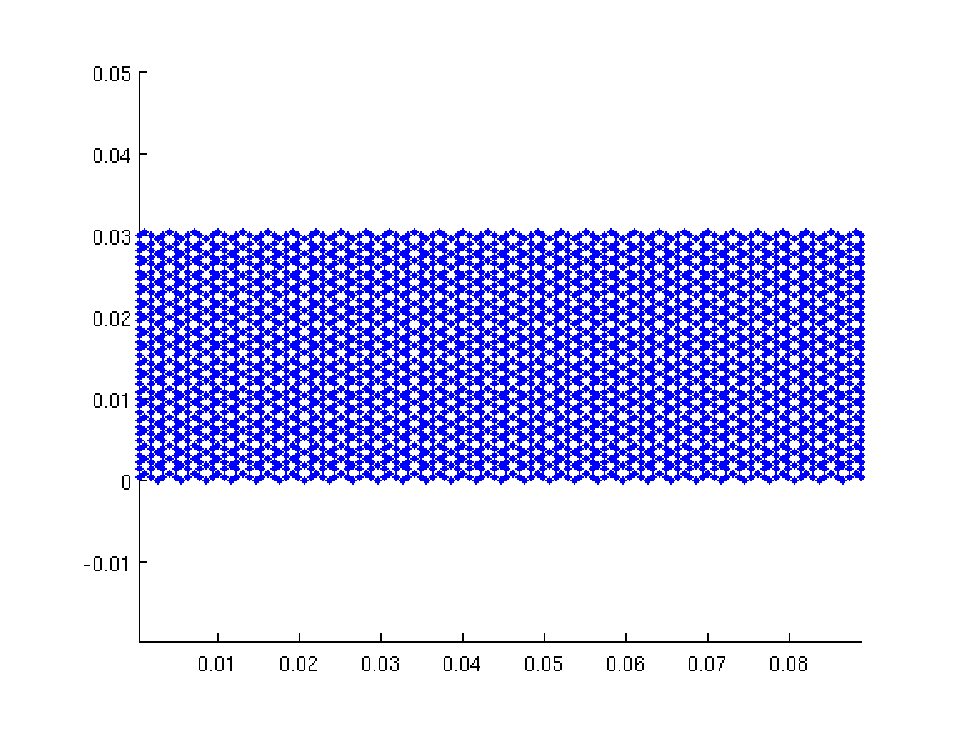
\includegraphics[width=0.8\textwidth]{MainPoreNetwork_01}
	\caption[]{Example geometry of the pore-space network. The used parameters were: {\tt n = 120}, {\tt m = 36} and {\tt l\textunderscore pore = 0.001} (given in meter). This resulted in network with $n_{pore} = 3162$ number of pores and $n_{node} = 2160$ number of nodes. The dimensions were $L_x = 0.09\ m$ and $L_y = 0.03\ m$ in $x$ and $y$ directions respectively.} 
	\label{fig:geometry}
\end{figure}

The result is the raw geometry of the pore network(see Figure \ref{fig:geometry}), which is used in the following for the calculation of flow and transport.

\begin{figure}[ht]
	\centering
	% Generated with LaTeXDraw 2.0.5
% Wed May 15 11:42:44 CEST 2013
% \usepackage[usenames,dvipsnames]{pstricks}
% \usepackage{epsfig}
% \usepackage{pst-grad} % For gradients
% \usepackage{pst-plot} % For axes
\scalebox{1} % Change this value to rescale the drawing.
{
\begin{pspicture}(0,-3.92)(13.329062,3.92)
\psline[linewidth=0.04cm](4.96,1.92)(7.96,1.92)
\psline[linewidth=0.04cm](4.96,-1.68)(7.96,-1.68)
\psline[linewidth=0.04cm](7.96,1.92)(9.9,0.12)
\psline[linewidth=0.04cm](7.96,-1.68)(9.86,0.12)
\psline[linewidth=0.04cm](3.04,0.12)(4.98,-1.68)
\psline[linewidth=0.04cm](3.08,0.12)(4.98,1.92)
\psline[linewidth=0.04cm,linestyle=dashed,dash=0.16cm 0.16cm](9.84,0.12)(12.84,0.12)
\psline[linewidth=0.04cm,linestyle=dashed,dash=0.16cm 0.16cm](0.06,0.1)(3.06,0.1)
\psline[linewidth=0.04cm,linestyle=dashed,dash=0.16cm 0.16cm](7.98,-1.68)(9.92,-3.48)
\psline[linewidth=0.04cm,linestyle=dashed,dash=0.16cm 0.16cm](3.04,3.72)(4.98,1.92)
\psline[linewidth=0.04cm,linestyle=dashed,dash=0.16cm 0.16cm](7.96,1.92)(9.86,3.72)
\psline[linewidth=0.04cm,linestyle=dashed,dash=0.16cm 0.16cm](3.08,-3.48)(4.98,-1.68)
\psline[linewidth=0.04cm,linestyle=dotted,dotsep=0.16cm](3.0,3.9)(3.0,-3.9)
\psline[linewidth=0.04cm,linestyle=dotted,dotsep=0.16cm](4.94,3.9)(4.94,-3.9)
\psline[linewidth=0.04cm,linestyle=dotted,dotsep=0.16cm](8.0,3.9)(8.0,-3.9)
\psline[linewidth=0.04cm,linestyle=dotted,dotsep=0.16cm](9.88,3.9)(9.88,-3.9)
\psline[linewidth=0.04cm,linestyle=dotted,dotsep=0.16cm](12.8,1.9)(0.0,1.9)
\psline[linewidth=0.04cm,linestyle=dotted,dotsep=0.16cm](12.8,-1.7)(0.0,-1.7)
\psline[linewidth=0.04cm,arrowsize=0.05291667cm 2.0,arrowlength=1.4,arrowinset=0.4]{<->}(12.4,1.8)(12.4,-1.6)
\usefont{T1}{ptm}{m}{n}
\rput(12.769688,1.105){{\tt m}}
\psline[linewidth=0.04cm,arrowsize=0.05291667cm 2.0,arrowlength=1.4,arrowinset=0.4]{<->}(3.1,3.0)(9.8,3.0)
\usefont{T1}{ptm}{m}{n}
\rput(6.4596877,3.385){{\tt n}}
\psline[linewidth=0.04cm,linestyle=dotted,dotsep=0.16cm](12.8,0.1)(0.0,0.1)
\usefont{T1}{ptm}{m}{n}
\rput(1.684375,1.145){pores}
\usefont{T1}{ptm}{m}{n}
\rput(1.6326562,-0.915){nodes}
\psline[linewidth=0.02cm,arrowsize=0.05291667cm 2.0,arrowlength=1.4,arrowinset=0.4]{->}(2.3,1.02)(3.68,0.82)
\psline[linewidth=0.02cm,arrowsize=0.05291667cm 2.0,arrowlength=1.4,arrowinset=0.4]{->}(2.28,1.18)(6.06,1.74)
\psline[linewidth=0.02cm,arrowsize=0.05291667cm 2.0,arrowlength=1.4,arrowinset=0.4]{->}(2.32,1.1)(8.66,1.06)
\psline[linewidth=0.02cm,arrowsize=0.05291667cm 2.0,arrowlength=1.4,arrowinset=0.4]{->}(2.2,-0.8)(3.0,-0.02)
\psline[linewidth=0.02cm,arrowsize=0.05291667cm 2.0,arrowlength=1.4,arrowinset=0.4]{->}(2.22,-0.86)(9.56,0.04)
\psline[linewidth=0.02cm,arrowsize=0.05291667cm 2.0,arrowlength=1.4,arrowinset=0.4]{->}(2.24,-0.94)(7.92,-1.6)
\psline[linewidth=0.02cm,arrowsize=0.05291667cm 2.0,arrowlength=1.4,arrowinset=0.4]{->}(2.2,-1.04)(4.74,-1.66)
\end{pspicture} 
}


	\caption{Schematic of the hexagonal pore structure.}
	\label{fig:PoreStructure}
\end{figure}

The parameters {\tt n} and {\tt m} need some further explanation since their values do not straight forwardly apply to the generated pore structure. The layout of the structure is a hexagonal honey-comb network of interconnected tubes having an angle of $\varphi = 120^{\circ}$. Here these tubes represent the pores and effects appearing on the nodes are neglected. The hexagonal grid has been chosen over a simpler square grid since the latter produces unphysical effects due to an over-regular structure \citep{Dupin2001}.

A schematic representation of the hexagonal layout of the pore network can be seen in Figure \ref{fig:PoreStructure}, where the dotted lines represent the hypothetical grid, along which the pores are arranged. The values {\tt n} and {\tt m} are therefore the number of these lines of this hypothetical square grid. A single hexagonal pore therefore needs {\tt n = 4} and {\tt m = 3}. Due to reasons regarding symmetry the parameter {\tt n} should always be a multiple of 4 and {\tt m} being a multiple of 2. 

As a result of this design decision, it is also not straight forward to compute the number of pores or the physical dimensions of the network, which are generated for a given {\tt n} and {\tt m}. Whereas the number of nodes is simply $ n_{node} = n\ m/2 $, the number of pores can be calculated according to $ n_{pore} = n/2 (m-1) + (n/2-1) \rm{ceil}(m/2)$, where $\rm{ceil}$ rounds towards minus infinity. The lenght $L_x$ and height $L_y$ of the generated pore network can be calculated according to $L_x = l_{pore} ((n/2 - 1)1.5) + 0.5$ and $L_y = (m - 1)\sin(\varphi)$. If the physical dimensions are given, the necessary number of elements can be computed according to $n = 4/3(L_x/l_{pore} - 0.5) + 2$ and $m = L_y/\sin(\varphi) + 1$. Both values should be rounded such that above conditions are meet.

\section{Assigning random pore radii to the geometry}

In the second step random pore radii are generated by the function {\tt getRadii.m} in order to get a heterogeneous pore space. The relevant parameters are

\begin{itemize}
	\item {\tt lambda\_x}, i.e. the correlation length $\lambda_x$ in the x-direction,
	\item {\tt lambda\_y}, i.e. the correlation length $\lambda_y$ in the y-direction,
	\item {\tt mu}, i.e. the expectation value $\mu$ of the random field,
	\item {\tt sigma2}, i.e. the variance $\sigma^2$ of the random field and
	\item {\tt func}, which defines the variogram function of the random field. 
	\item The type of the one-point distribution.
\end{itemize}

These parameters are again grouped in a {\tt struct} variable called {\tt RadiiCoeffs}. The return value of the {\tt getRadii.m} function is a list containing the pore radii of every pore.

\begin{figure}[ht]
	\centering
	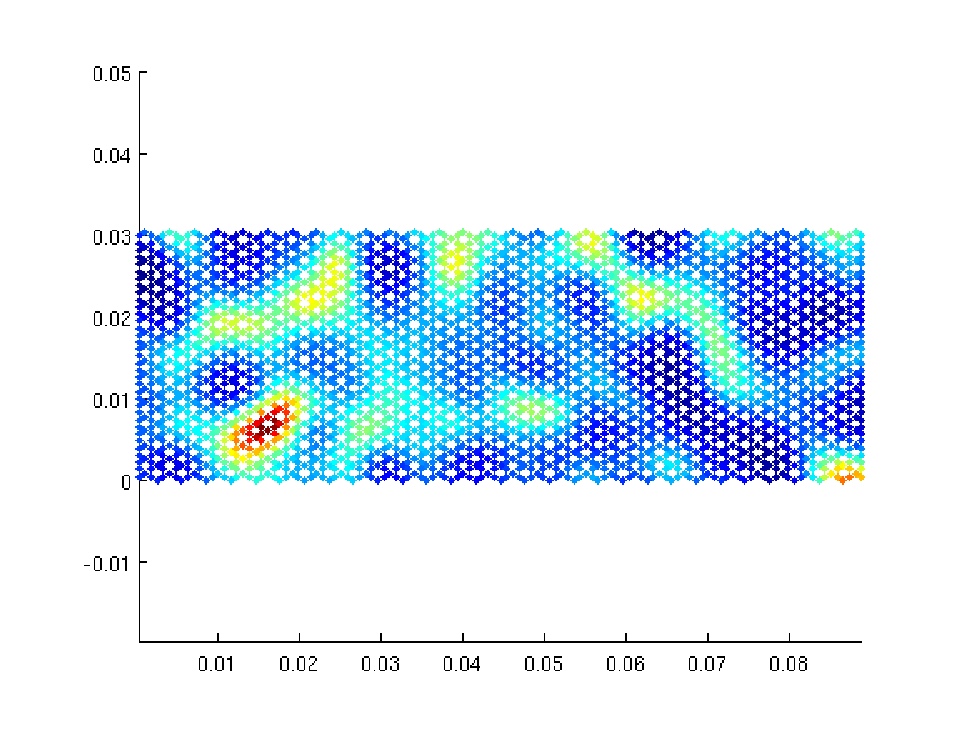
\includegraphics[width=0.8\textwidth]{MainPoreNetwork_02}
	\caption[]{Example geometry of the pore-space network with heterogeneous distributed pore radii. The used parameters were: $\lambda_x = \lambda_y = 0.005$, $\mu = 0.16\ 10^{-3}$ and $\sigma^2 = 5\ 10^{-9}$. The field was log-normally distributed and had a Gaussian variogram.}
	\label{fig:radii}
\end{figure}

The function uses a random field generator, which can provide random values for the pores. The position is taken to be at the center of each pore. The field generator can provide both a normal as well as a log-normal distribution for the point values. For the variogram several model functions can be generated: a Gaussian, an exponential, a power law as well as a truncated power law. The generator can also provide isotropic and anisotropic fields.

\section{Computing the flow field}

In the third step the velocity field is generated and assigned to every pore $j$ in the network by the function {\tt getFlow.m}. The relevant parameters are

\begin{itemize}
	\item  {\tt delta\_p}, which is the pressure drop $\Delta P$ along the whole geometry.
\end{itemize}

Since the flow direction is assumed to be from the left to the right, $\Delta p$ is defined accordingly. The flow parameters are again grouped in a {\tt struct} variable called {\tt FlowCoeffs}. The return value of the {\tt getFlow.m} function is a list containing the flow velocities in every pore.

\begin{figure}[ht]
	\centering
	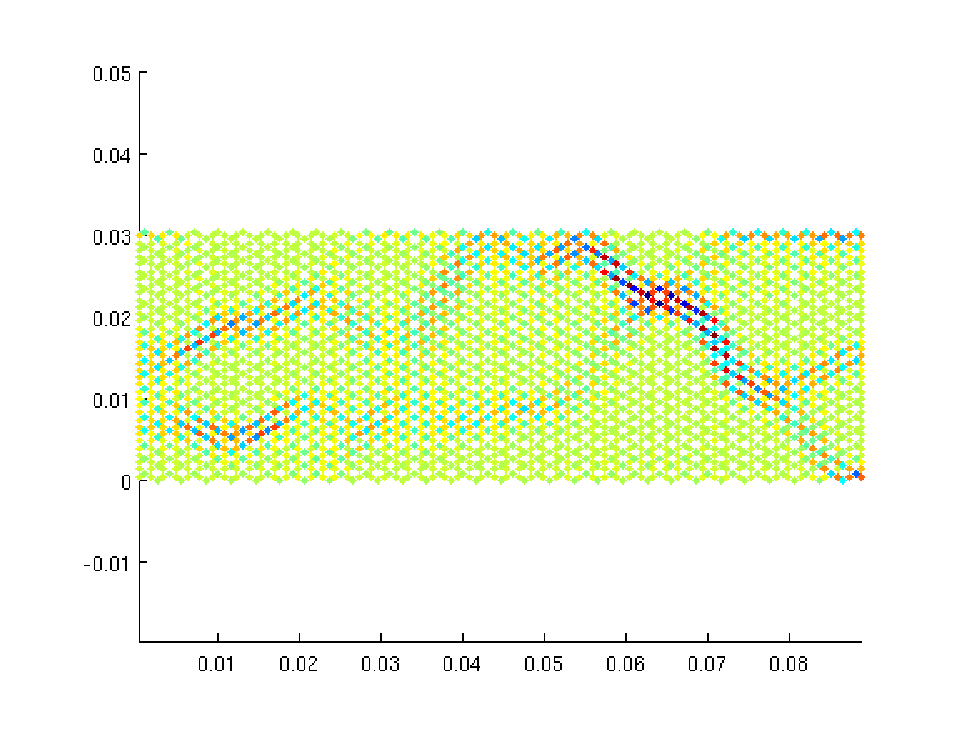
\includegraphics[width=0.8\textwidth]{MainPoreNetwork_03}
	\caption[]{Example geometry of the pore-space network with heterogeneous distributed pore radii. The used parameters were: $\lambda_x = \lambda_y = 0.005$, $\mu = 0.16\ 10^{-3}$ and $\sigma^2 = 5\ 10^{-9}$. The field was log-normally distributed and had a Gaussian variogram.}
	\label{fig:flow}
\end{figure}

For the solution the Hagen Poiseuille equation is used in order to compute the volumetric flow in each pore:

$$
	q_j = \frac{\pi r^4_j}{8 \nu} \frac{\Delta p_j}{l_{pore}}.
$$

Here $\nu$ is the dynamic viscosity of water and $\Delta p_j $ is the pressure drop along pore $j$. Interpreting above equation by using Darcy's law we get $K = (\pi r^4_j/8 \nu l_{pore})$ as the conductivity of each pore. Mass conservation is achieved by using Kirchhoff's law, i.e. $q_{j,1} + q_{j,2} + q_{j,3} = 0$ in case of a hexagonal grid (see Figure \ref{fig:PoreStructure}). By virtue of Kirchoff's law and using above equation one can derive a system of $n_{pore}$ equations, which can be solved for the $n_{pore}$ unknowns of $q_j$.

The flow is then used in order to determine the water velocity in each pore $j$ according to

$$ 
	u_j = \frac{q_j}{\pi r_j^2}. 
$$ 

These data are then used in order to determine the advective transport of each species.

\section{Solving the transport}

In the fourth step the time-dependent (reactive) transport is solved for a number of $n_{spec}$ chemical species in each pore $j$ in the function {\tt getTransport.m}. The relevant parameters used for the solution of the transport are

\begin{itemize}
	\item {\tt t\_end}, which is the length of the time interval,
	\item {\tt t\_0}, which is the beginning of the time interval,
	\item {\tt dt}, which is the length of the step size $\Delta t$ and
	\item {\tt spec\_no}, which is the number $n_{spec}$ of chemical species.
\end{itemize}

These parameters are again grouped in a {\tt struct} variable called {\tt TransportCoeffs}. The return value of the {\tt getTransport.m} function is a list containing the concentration values of every species $i$ in every pore $j$.

\begin{figure}[ht]
	\subfigure
	{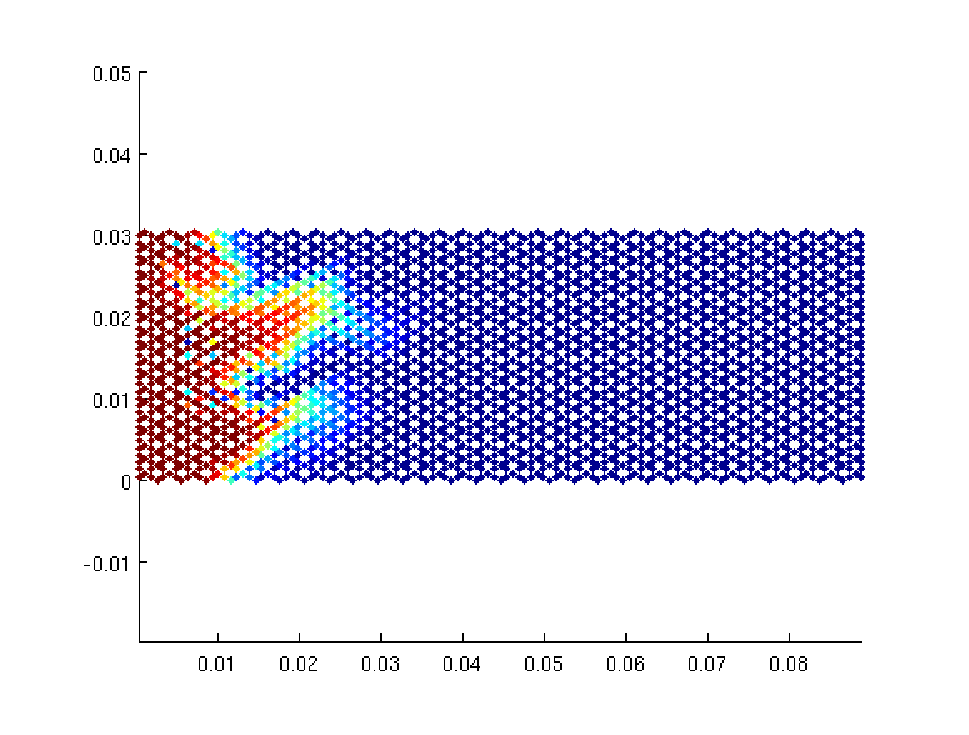
\includegraphics[width=0.5\textwidth]{MainPoreNetwork_04}}\hfill
	\subfigure
	{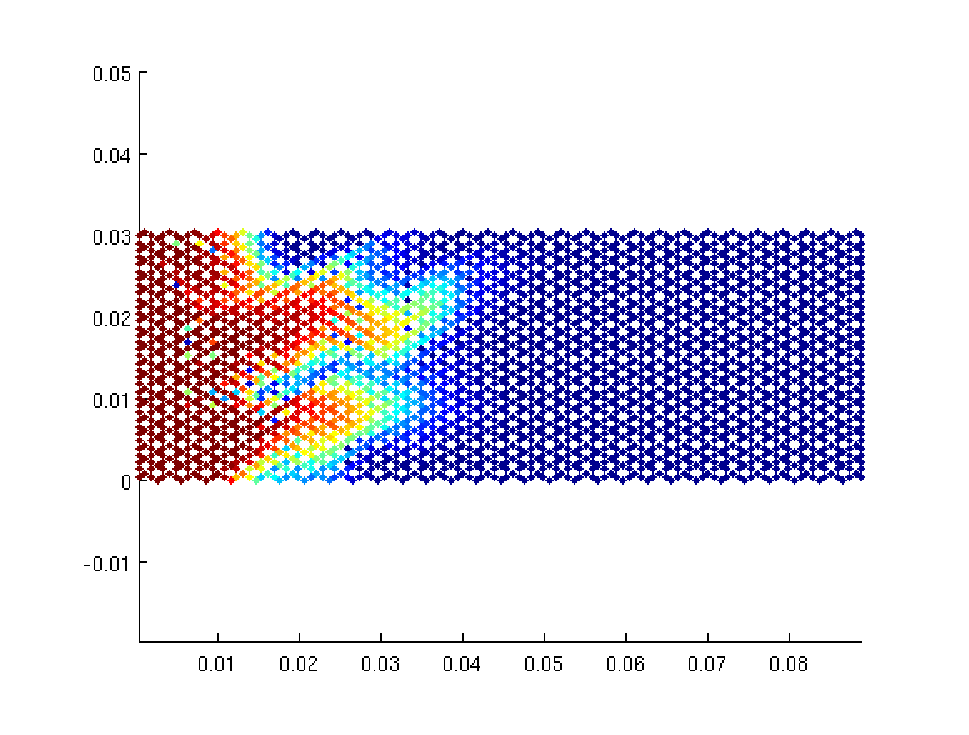
\includegraphics[width=0.5\textwidth]{MainPoreNetwork_05}}\\
	\subfigure
	{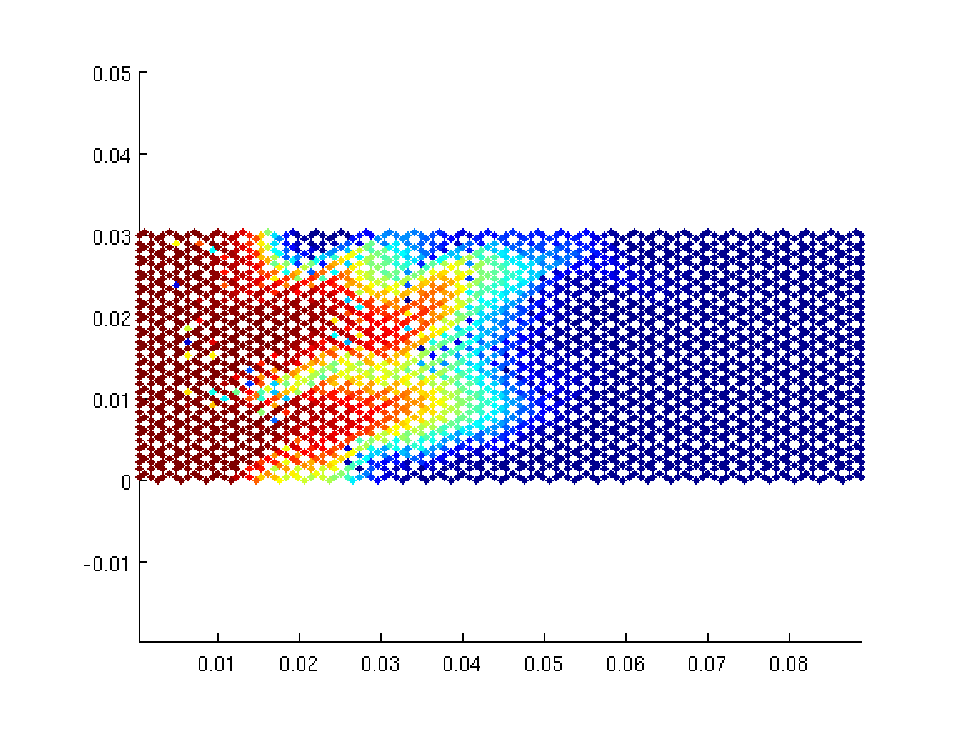
\includegraphics[width=0.5\textwidth]{MainPoreNetwork_06}}\hfill
	\subfigure
	{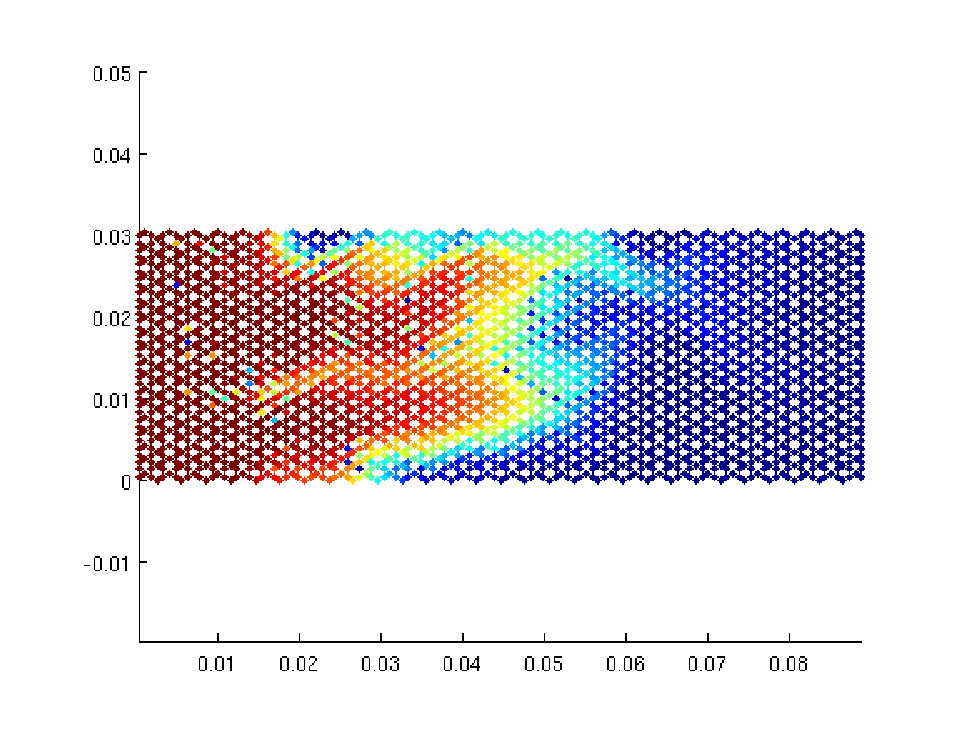
\includegraphics[width=0.5\textwidth]{MainPoreNetwork_07}}
	\caption{Transport of a conservative tracer at four consecutive time steps.}
	\label{fig:transport}
\end{figure}

The transport step is solved using the advection-diffusion-reaction equation within each pore $j$, i.e.

\begin{equation}\label{eq:adr_equation}
	\frac{\partial}{\partial t} c_{i,j} = - \frac{\partial}{\partial x_L} \cdot ( u_j c_{i,j}) + D_i \left( \frac{\partial^2}{\partial x_L^2} + \frac{\partial^2}{\partial x_T^2} \right) c_{i,j} + r_{i,j}.
\end{equation}


Here $t$ is the time, $c_{i,j}$ is the concentration of species $i$ in pore $j$, $D_i$ is the diffusion coefficient of each species and $R_{i,j}$ the respective production and consumption rate. Several methods can be employed for the reaction part. The directions $x_L$ and $x_T$ are the longitudinal and transversal directions within each pore. Two different scenarios are possible according to the hexagonal geometry (see Figure \ref{fig:PoreStructure}): (i) a horizontal pore, were $x_L = x$ and $x_T = y$ as well as (ii) an inclined pore, were $x_L$ and $x_T$ are inclined, too.

Instead of the full two-dimensional system given by Equation (\ref{eq:adr_equation}) we only solve a one-dimensional system averaged along the width of the pore. This sytem is given by the following expression

\begin{equation}\label{eq:adr_equation_av}
	\frac{\partial}{\partial t} {\bf C}_{\rm{j}} = - \frac{\partial}{\partial x_L} \cdot ( {\bf U}_{\rm{j}} {\bf C}_{\rm{j}}) + {\bf D} \frac{\partial^2}{\partial x_L^2} {\bf C}_{\rm{j}} + {\bf R}_{\rm{j}}.
\end{equation}

Here ${\bf C}_{\rm{j}}$ is the list of the averaged concentration of all species and ${\bf U}_{\rm{j}}$, ${\bf D}$ and ${\bf R}_{\rm{j}}$ are lists of the appropriate velocity, diffusion and reaction components. For a derivation of this coefficient functions we refer to \citep{Hesse2010}.

In order to solve Equation (\ref{eq:adr_equation_av}) for every pore a simple operator splitting procedure is applied, where the different terms like advection, longitudinal diffusion as well as reaction are solved successively. For the discretization of the time derivative a simple explicit Euler scheme is employed, i.e.

$$
	\frac{\partial}{\partial t} {\bf C}_{\rm{j}} \approx \frac{\Delta {\bf C}_{\rm{j}}}{\Delta t} = \frac{{\bf C}_{\rm{j}}^{\rm{n}} - {\bf C}_{\rm{j}}^{\rm{n} - 1}}{\Delta t} .
$$

In order to avoid unstable solutions, which may arise with this method, the Courant-Friedrichs-Levy conditions must be meet. 

\paragraph*{Advection}

According to Equation (\ref{eq:adr_equation_av}) we get for the advection the following expression

$$
	 \left( \frac{\partial}{\partial t} {\bf C}_{\rm{j}} \right)_{\rm{adv}} = - \frac{\partial}{\partial x_L} \cdot ({\bf U}_{\rm{j}} {\bf C}_{\rm{j}}).
$$

Like the time derivative, the spatial derivative in this expression is also approximated by using a difference method, i.e. the differential is replaced with a difference, leading to the following expression

\begin{subequations}
\begin{align}
	 \left( \Delta {\bf C}_{\rm{j}} \right)_{\rm{adv}} & = - \frac{\Delta t}{ \Delta x } {\bf U}_{\rm{j}} ({\bf C}^{\rm{n} - 1}_{\rm{in, j}} - {\bf C}^{\rm{n} - 1}_{\rm{j}}) \\
	 {\bf C}_{\rm{in}} & = \frac{\sum q_k {\bf C}_k}{ \sum q_k } 
\end{align}
\end{subequations}

Here the ${\bf C}_{\rm{in, j}}$ is the list of inlet concentrations for each pore $j$. Due to the hexagonal geometry the calculation depends on the type of node.

\begin{figure}[ht]
	\centering
	% Generated with LaTeXDraw 2.0.5
% Tue Jul 30 10:20:20 CEST 2013
% \usepackage[usenames,dvipsnames]{pstricks}
% \usepackage{epsfig}
% \usepackage{pst-grad} % For gradients
% \usepackage{pst-plot} % For axes
\scalebox{1} % Change this value to rescale the drawing.
{
\begin{pspicture}(0,-3.02)(13.0,3.02)
\psline[linewidth=0.04cm](2.8,0.2)(4.4,0.2)
\psline[linewidth=0.04cm](2.8,-0.2)(4.4,-0.2)
\psline[linewidth=0.04cm](4.6,0.0)(5.6,0.8)
\psline[linewidth=0.04cm](5.58,1.2)(7.18,1.2)
\psline[linewidth=0.04cm](5.6,0.8)(7.2,0.8)
\psline[linewidth=0.04cm](5.6,-1.2)(7.2,-1.2)
\psline[linewidth=0.04cm](5.6,-0.8)(7.2,-0.8)
\psline[linewidth=0.04cm](4.6,0.0)(5.6,-0.8)
\psline[linewidth=0.04cm](0.0,-1.2)(1.6,-1.2)
\psline[linewidth=0.04cm](0.0,-0.8)(1.6,-0.8)
\psline[linewidth=0.04cm](1.58,0.8)(2.58,0.0)
\psline[linewidth=0.04cm](1.58,-0.8)(2.58,0.0)
\psline[linewidth=0.04cm](0.0,1.2)(1.6,1.2)
\psline[linewidth=0.04cm](0.0,0.8)(1.6,0.8)
\psline[linewidth=0.04cm](4.38,-0.2)(5.38,-1.0)
\psline[linewidth=0.04cm](4.62,-2.0)(5.62,-1.2)
\psline[linewidth=0.04cm](4.38,-1.8)(5.38,-1.0)
\psline[linewidth=0.04cm](2.8,-1.8)(4.4,-1.8)
\psline[linewidth=0.04cm](2.8,-2.2)(4.4,-2.2)
\psline[linewidth=0.04cm](1.82,-1.0)(2.82,-0.2)
\psline[linewidth=0.04cm](1.82,-1.0)(2.82,-1.8)
\psline[linewidth=0.04cm](1.6,-1.2)(2.6,-2.0)
\psline[linewidth=0.04cm](1.82,-3.0)(2.82,-2.2)
\psline[linewidth=0.04cm](1.6,-2.78)(2.6,-1.98)
\psline[linewidth=0.04cm](4.38,-2.2)(5.38,-3.0)
\psline[linewidth=0.04cm](4.6,-2.0)(5.6,-2.8)
\psline[linewidth=0.04cm](4.38,0.2)(5.38,1.0)
\psline[linewidth=0.04cm](1.8,1.0)(2.8,0.2)
\psline[linewidth=0.04cm](4.6,2.0)(5.6,1.2)
\psline[linewidth=0.04cm](4.38,1.8)(5.38,1.0)
\psline[linewidth=0.04cm](1.58,1.2)(2.58,2.0)
\psline[linewidth=0.04cm](1.78,1.0)(2.78,1.8)
\pscircle[linewidth=0.04,linecolor=red,dimen=outer](8.23,0.01){0.4}
\pscircle[linewidth=0.04,linecolor=red,dimen=outer](5.47,1.01){0.4}
\pscircle[linewidth=0.04,linecolor=red,dimen=outer](8.25,2.03){0.4}
\pscircle[linewidth=0.04,linecolor=red,dimen=outer](5.47,-0.99){0.4}
\pscircle[linewidth=0.04,linecolor=blue,dimen=outer](7.31,1.03){0.4}
\pscircle[linewidth=0.04,linecolor=blue,dimen=outer](7.35,-0.99){0.4}
\pscircle[linewidth=0.04,linecolor=blue,dimen=outer](4.51,0.03){0.4}
\pscircle[linewidth=0.04,linecolor=blue,dimen=outer](4.53,2.01){0.4}
\psline[linewidth=0.04cm](2.78,1.8)(4.38,1.8)
\psline[linewidth=0.04cm](2.78,2.2)(4.38,2.2)
\psline[linewidth=0.04cm](4.36,2.2)(5.36,3.0)
\psline[linewidth=0.04cm](4.58,2.0)(5.58,2.8)
\psline[linewidth=0.04cm](1.8,3.0)(2.8,2.2)
\psline[linewidth=0.04cm](1.58,2.8)(2.58,2.0)
\psline[linewidth=0.04cm](7.2,0.8)(8.2,0.0)
\psline[linewidth=0.04cm](7.18,-1.2)(8.18,-2.0)
\psline[linewidth=0.04cm](7.16,1.2)(8.16,2.0)
\psline[linewidth=0.04cm](7.18,-0.8)(8.18,0.0)
\psline[linewidth=0.04cm](7.38,1.0)(8.38,1.8)
\psline[linewidth=0.04cm](8.38,1.8)(9.98,1.8)
\psline[linewidth=0.04cm](8.38,2.2)(9.98,2.2)
\psline[linewidth=0.04cm](8.38,0.2)(9.98,0.2)
\psline[linewidth=0.04cm](8.38,-0.2)(9.98,-0.2)
\psline[linewidth=0.04cm](7.4,1.0)(8.4,0.2)
\psline[linewidth=0.04cm](7.4,-1.0)(8.4,-1.8)
\psline[linewidth=0.04cm](8.38,-1.8)(9.98,-1.8)
\psline[linewidth=0.04cm](7.38,-1.0)(8.38,-0.2)
\psline[linewidth=0.04cm](7.38,3.0)(8.38,2.2)
\psline[linewidth=0.04cm](7.16,2.8)(8.16,2.0)
\psline[linewidth=0.04cm](8.38,-2.2)(9.98,-2.2)
\psline[linewidth=0.04cm](7.16,-2.8)(8.16,-2.0)
\psline[linewidth=0.04cm](5.58,2.8)(7.18,2.8)
\psline[linewidth=0.04cm](7.38,-3.0)(8.38,-2.2)
\psline[linewidth=0.04cm](5.58,-2.8)(7.18,-2.8)
\psline[linewidth=0.04cm](9.96,2.2)(10.96,3.0)
\psline[linewidth=0.04cm](9.96,0.2)(10.96,1.0)
\psline[linewidth=0.04cm](9.96,-1.8)(10.96,-1.0)
\psline[linewidth=0.04cm](11.38,1.2)(12.98,1.2)
\psline[linewidth=0.04cm](9.98,1.8)(10.98,1.0)
\psline[linewidth=0.04cm](9.96,-0.2)(10.96,-1.0)
\psline[linewidth=0.04cm](11.38,0.8)(12.98,0.8)
\psline[linewidth=0.04cm](11.38,-0.8)(12.98,-0.8)
\psline[linewidth=0.04cm](11.38,-1.2)(12.98,-1.2)
\psline[linewidth=0.04cm](10.38,2.0)(11.38,1.2)
\psline[linewidth=0.04cm](10.4,0.0)(11.4,-0.8)
\psline[linewidth=0.04cm](9.96,-2.2)(10.96,-3.0)
\psline[linewidth=0.04cm](10.4,-1.98)(11.4,-2.78)
\psline[linewidth=0.04cm](10.4,-2.0)(11.4,-1.2)
\psline[linewidth=0.04cm](10.4,0.0)(11.4,0.8)
\psline[linewidth=0.04cm](10.38,2.0)(11.38,2.8)
\pscircle[linewidth=0.04,linecolor=red,dimen=outer](8.21,-1.99){0.4}
\pscircle[linewidth=0.04,linecolor=blue,dimen=outer](4.49,-1.97){0.4}
\end{pspicture} 
}


	\caption{The two different node types of the hexagonal geometry structure.}
	\label{fig:PoreStructure02}
\end{figure}

Two different types of nodes can be distinguished (see Figure \ref{fig:PoreStructure02}). The first type is where a horizontal pore is branching into two inclined pores. Every inclined pore therefore has only one inlet and the concentration is divided according to the fluxes. The second type of node is where two inclined pores merge into one horizontal pore. Here the inlet concentration is derived by summing up both predecessing concentration according to the fluxes.  

\paragraph*{Longitudinal Diffusion}

According to Equation (\ref{eq:adr_equation_av}) we get for the longitudinal diffusion the following expression

$$
	 \left( \frac{\partial}{\partial t} {\bf C}_{\rm{j}} \right)_{\rm{dif_L}} = {\bf D} \frac{\partial^2}{\partial x_L^2} {\bf C}_{\rm{j}}.
$$

Like in case of the advective flux we chose again a difference approximation leading to the following expression

$$
	\left( \Delta {\bf C}_{\rm{j}} \right)_{\rm{dif_L}} =  \Delta t {\bf D} \frac{ {\bf C}^{\rm{n} - 1}_{\rm{j-1}}  - 2 {\bf C}^{\rm{n} - 1}_{\rm{j}} + {\bf C}^{\rm{n} - 1}_{\rm{j-1}} }{\Delta x^2/2 },
$$

where ${\bf C}_{\rm{j-1}}$ and ${\bf C}_{\rm{j+1}}$ are the concentrations at the upstream and downstream nodes respectively. 

\paragraph*{Transversal Diffusion}

No transversal diffusion is featured in Equation (\ref{eq:adr_equation_av}) due to the averaging across the width of the pore.

\begin{figure}[ht]
	\centering
	% Generated with LaTeXDraw 2.0.5
% Tue Jul 30 14:03:05 CEST 2013
% \usepackage[usenames,dvipsnames]{pstricks}
% \usepackage{epsfig}
% \usepackage{pst-grad} % For gradients
% \usepackage{pst-plot} % For axes
\scalebox{1} % Change this value to rescale the drawing.
{
\begin{pspicture}(0,-4.02)(8.62,4.02)
\psline[linewidth=0.04cm](5.4,2.4)(8.6,2.4)
\psline[linewidth=0.04cm](3.2,3.6)(5.2,2.0)
\psline[linewidth=0.04cm](5.4,1.6)(8.6,1.6)
\psline[linewidth=0.04cm](3.4,4.0)(5.4,2.4)
\psline[linewidth=0.04cm](3.4,0.0)(5.4,1.6)
\psline[linewidth=0.04cm](3.2,0.4)(5.2,2.0)
\psline[linewidth=0.04cm](3.4,0.0)(5.4,-1.6)
\psline[linewidth=0.04cm](5.4,-1.6)(8.6,-1.6)
\psline[linewidth=0.04cm](5.4,-2.4)(8.6,-2.4)
\psline[linewidth=0.04cm](0.0,0.4)(3.2,0.4)
\psline[linewidth=0.04cm](0.0,-0.4)(3.2,-0.4)
\psline[linewidth=0.04cm](3.18,-0.4)(5.18,-2.0)
\psline[linewidth=0.04cm](3.42,-4.0)(5.42,-2.4)
\psline[linewidth=0.04cm](3.18,-3.6)(5.18,-2.0)
\psline[linewidth=0.04cm,linestyle=dashed,dash=0.16cm 0.16cm](5.4,2.0)(8.6,2.0)
\psline[linewidth=0.04cm,linestyle=dashed,dash=0.16cm 0.16cm](3.3,3.8)(5.3,2.2)
\psline[linewidth=0.04cm,linestyle=dashed,dash=0.16cm 0.16cm](0.0,0.0)(3.2,0.0)
\psline[linewidth=0.04cm,linestyle=dashed,dash=0.16cm 0.16cm](5.4,-2.0)(8.6,-2.0)
\psline[linewidth=0.04cm,linestyle=dashed,dash=0.16cm 0.16cm](3.3,0.2)(5.3,1.8)
\psline[linewidth=0.04cm,linestyle=dashed,dash=0.16cm 0.16cm](3.3,-3.8)(5.3,-2.2)
\psline[linewidth=0.04cm,linestyle=dashed,dash=0.16cm 0.16cm](3.3,-0.2)(5.3,-1.8)
\pscircle[linewidth=0.04,linecolor=red,dimen=outer](5.3,2.0){0.8}
\pscircle[linewidth=0.04,linecolor=red,dimen=outer](5.3,-2.0){0.8}
\pscircle[linewidth=0.04,linecolor=blue,dimen=outer](3.2,0.0){0.8}
\usefont{T1}{ptm}{m}{n}
\rput(2.559375,1.065){\color{blue}Type I node}
\usefont{T1}{ptm}{m}{n}
\rput(6.659375,3.085){\color{red}Type II node}
\usefont{T1}{ptm}{m}{n}
\rput(6.579375,-0.955){\color{red}Type II node}
\end{pspicture} 
}


	\caption{Discrimination of upper and lower pore regions in order to emulate transversal diffusion.}
	\label{fig:PoreStructure03}
\end{figure}

We can however, define an upper and a lower concentration for each pore $j$ (see Figure \ref{fig:PoreStructure03}) leading to the following approximation of the transversal diffusion

$$
	 \left( \frac{\partial}{\partial t} {\bf C}_{\rm{j}} \right)_{\rm{dif_T}} = {\bf D} \frac{\partial^2}{\partial x_T^2} {\bf C}_{\rm{j}}.
$$

Like in case of the longitudinal diffusional flux we chose again a difference approximation leading to the following expression

$$
	\left( \Delta {\bf C}_{\rm{j}} \right)_{\rm{dif_T}} = \Delta t {\bf D} \frac{\pi^2}{4} \frac{ \left( {\bf C}^{\rm{n} - 1}_{\rm{up,j}} - {\bf C}^{\rm{n} - 1}_{\rm{down,j}} \right)}{\Delta y^2_{\rm{j}}/2},
$$

where $\Delta y_{\rm{j}}$ is the width of the pore $j$ and ${\bf C}_{\rm{up,j}}$ and ${\bf C}_{\rm{down,j}}$ are the concentrations at the upper and lower part of the pore $j$ respectively. 

To fully implement upper and lower pore regions the advective part had to be adapted as well. The Kirchoff rule for the different nodes have therefore to be rewritten dependent on the node type.

\begin{figure}[ht]
	\centering
	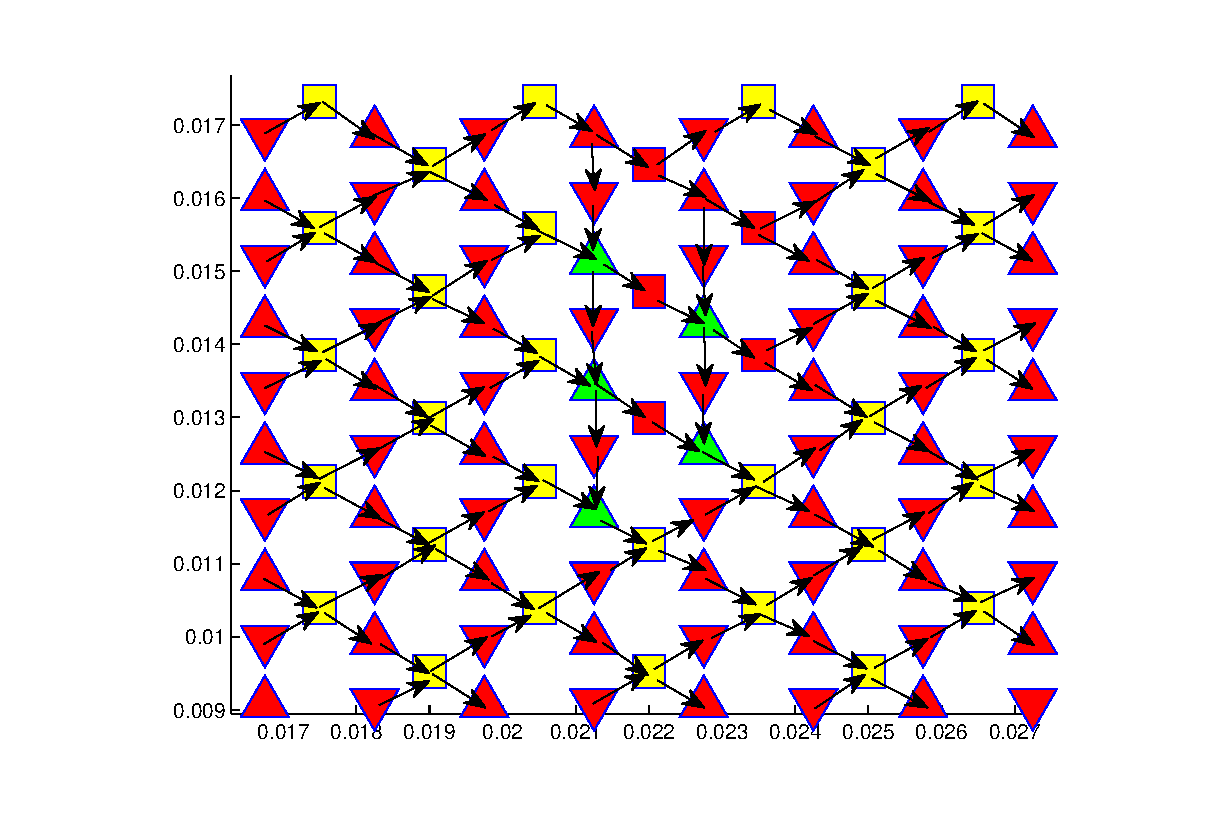
\includegraphics[width=0.8\textwidth]{node_types_02}
	\caption[]{Graphical representation of the different node types. The color of the pore denotes the type of inlet node, i.e. the node upstream of the pore. Yellow pores are straight pores with two inlets. Green pores are tilted pores with two inlets. Red pores are pores with one inlet. The arows indicate the flow direction.} 
	\label{fig:node_types}
\end{figure}

Even in a simple hexagonal structure with uniform mean average flow, the situation is complex due to different flow paths that the solute can take (see Figure \ref{fig:node_types}). For the geometry as well as the used boundary conditions several types of nodes can therefore be distinguished. 

\begin{figure}[ht]
	\subfigure
	{% Generated with LaTeXDraw 2.0.8
% Tue May 05 15:08:35 CEST 2015
% \usepackage[usenames,dvipsnames]{pstricks}
% \usepackage{epsfig}
% \usepackage{pst-grad} % For gradients
% \usepackage{pst-plot} % For axes
\scalebox{1} % Change this value to rescale the drawing.
{
\begin{pspicture}(0,-3.415)(6.9396877,3.435)
\psline[linewidth=0.04cm](3.6196876,2.685)(6.9196873,2.685)
\psline[linewidth=0.04cm](3.7196875,2.205)(6.9196873,2.205)
\psline[linewidth=0.04cm](1.7196875,0.605)(3.7196875,2.205)
\psline[linewidth=0.04cm](1.5196875,1.005)(3.6196876,2.685)
\psline[linewidth=0.04cm](1.7196875,0.605)(3.7196875,-0.995)
\psline[linewidth=0.04cm](3.7196875,-0.995)(6.9196873,-0.995)
\psline[linewidth=0.04cm](3.7196875,-1.795)(6.9196873,-1.795)
\psline[linewidth=0.04cm](1.4996876,0.205)(3.4996874,-1.395)
\psline[linewidth=0.04cm](1.7396874,-3.395)(3.7396874,-1.795)
\psline[linewidth=0.04cm](1.4996876,-2.995)(3.4996874,-1.395)
\psline[linewidth=0.04cm,linestyle=dashed,dash=0.16cm 0.16cm](3.7196875,2.425)(6.9196873,2.425)
\psline[linewidth=0.04cm,linestyle=dashed,dash=0.16cm 0.16cm](3.7196875,-1.395)(6.9196873,-1.395)
\psline[linewidth=0.04cm,linestyle=dashed,dash=0.16cm 0.16cm](1.6196876,0.805)(3.6196876,2.405)
\psline[linewidth=0.04cm,linestyle=dashed,dash=0.16cm 0.16cm](1.6196876,-3.195)(3.6196876,-1.595)
\psline[linewidth=0.04cm,linestyle=dashed,dash=0.16cm 0.16cm](1.6196876,0.405)(3.6196876,-1.195)
\pscircle[linewidth=0.04,linecolor=red,dimen=outer](3.6796875,2.485){0.8}
\pscircle[linewidth=0.04,linecolor=blue,dimen=outer](1.5196875,0.605){0.8}
\usefont{T1}{ptm}{m}{n}
\rput(0.8684375,1.67){\color{blue}Type I node}
\usefont{T1}{ptm}{m}{n}
\rput(5.3284373,3.25){\color{red}Type II node}
\end{pspicture} 
}

} \hfill
	\subfigure
	{% Generated with LaTeXDraw 2.0.8
% Thu May 28 10:02:38 CEST 2015
% \usepackage[usenames,dvipsnames]{pstricks}
% \usepackage{epsfig}
% \usepackage{pst-grad} % For gradients
% \usepackage{pst-plot} % For axes
\scalebox{1} % Change this value to rescale the drawing.
{
\begin{pspicture}(0,-4.02)(8.62,4.02)
\psline[linewidth=0.04cm](5.4,2.4)(8.6,2.4)
\psline[linewidth=0.04cm](3.2,3.6)(5.2,2.0)
\psline[linewidth=0.04cm](5.4,1.6)(8.6,1.6)
\psline[linewidth=0.04cm](3.4,4.0)(5.4,2.4)
\psline[linewidth=0.04cm](3.4,0.0)(5.4,1.6)
\psline[linewidth=0.04cm](3.2,0.4)(5.2,2.0)
\psline[linewidth=0.04cm](3.4,0.0)(5.4,-1.6)
\psline[linewidth=0.04cm](5.4,-1.6)(8.6,-1.6)
\psline[linewidth=0.04cm](5.4,-2.4)(8.6,-2.4)
\psline[linewidth=0.04cm](0.0,0.4)(3.2,0.4)
\psline[linewidth=0.04cm](0.0,-0.4)(3.2,-0.4)
\psline[linewidth=0.04cm](3.18,-0.4)(5.18,-2.0)
\psline[linewidth=0.04cm](3.42,-4.0)(5.42,-2.4)
\psline[linewidth=0.04cm](3.18,-3.6)(5.18,-2.0)
\psline[linewidth=0.04cm,linestyle=dashed,dash=0.16cm 0.16cm](5.4,2.0)(8.6,2.0)
\psline[linewidth=0.04cm,linestyle=dashed,dash=0.16cm 0.16cm](3.3,3.8)(5.3,2.2)
\psline[linewidth=0.04cm,linestyle=dashed,dash=0.16cm 0.16cm](0.0,0.0)(3.2,0.0)
\psline[linewidth=0.04cm,linestyle=dashed,dash=0.16cm 0.16cm](5.4,-2.0)(8.6,-2.0)
\psline[linewidth=0.04cm,linestyle=dashed,dash=0.16cm 0.16cm](3.3,0.2)(5.3,1.8)
\psline[linewidth=0.04cm,linestyle=dashed,dash=0.16cm 0.16cm](3.3,-3.8)(5.3,-2.2)
\psline[linewidth=0.04cm,linestyle=dashed,dash=0.16cm 0.16cm](3.3,-0.2)(5.3,-1.8)
\pscircle[linewidth=0.04,linecolor=red,dimen=outer](5.3,-2.0){0.8}
\usefont{T1}{ptm}{m}{n}
\rput(2.258125,0.925){\color{blue}Type III node}
\usefont{T1}{ptm}{m}{n}
\rput(6.678125,2.945){\color{red}Type IV node}
\psline[linewidth=0.02cm,arrowsize=0.05291667cm 2.0,arrowlength=1.4,arrowinset=0.4]{->}(4.64,2.86)(5.38,2.24)
\psline[linewidth=0.02cm,arrowsize=0.05291667cm 2.0,arrowlength=1.4,arrowinset=0.4]{->}(4.56,2.64)(5.26,2.06)
\psline[linewidth=0.02cm,arrowsize=0.05291667cm 2.0,arrowlength=1.4,arrowinset=0.4]{->}(5.48,2.22)(6.48,2.22)
\psline[linewidth=0.02cm,arrowsize=0.05291667cm 2.0,arrowlength=1.4,arrowinset=0.4]{->}(5.48,1.82)(6.48,1.82)
\psline[linewidth=0.02cm,arrowsize=0.05291667cm 2.0,arrowlength=1.4,arrowinset=0.4]{->}(4.54,1.36)(5.28,1.9)
\psline[linewidth=0.02cm,arrowsize=0.05291667cm 2.0,arrowlength=1.4,arrowinset=0.4]{->}(4.62,1.12)(5.38,1.74)
\psline[linewidth=0.02cm,arrowsize=0.05291667cm 2.0,arrowlength=1.4,arrowinset=0.4]{->}(2.18,0.22)(3.18,0.22)
\psline[linewidth=0.02cm,arrowsize=0.05291667cm 2.0,arrowlength=1.4,arrowinset=0.4]{->}(2.18,-0.18)(3.18,-0.18)
\psline[linewidth=0.02cm,arrowsize=0.05291667cm 2.0,arrowlength=1.4,arrowinset=0.4]{->}(3.32,0.36)(3.98,0.9)
\psline[linewidth=0.02cm,arrowsize=0.05291667cm 2.0,arrowlength=1.4,arrowinset=0.4]{->}(3.4,0.14)(4.1,0.7)
\psline[linewidth=0.02cm,arrowsize=0.05291667cm 2.0,arrowlength=1.4,arrowinset=0.4]{->}(3.44,-0.18)(4.08,-0.72)
\psline[linewidth=0.02cm,arrowsize=0.05291667cm 2.0,arrowlength=1.4,arrowinset=0.4]{->}(3.28,-0.34)(3.98,-0.9)
\usefont{T1}{ptm}{m}{n}
\rput(6.658125,-1.075){\color{red}Type IV node}
\pscircle[linewidth=0.04,linecolor=red,dimen=outer](5.3,2.0){0.8}
\usefont{T1}{ptm}{m}{n}
\rput(6.067656,2.005){\psframebox*[framesep=0, boxsep=false,fillcolor=white] {3}}
\usefont{T1}{ptm}{m}{n}
\rput(4.7985935,2.585){\psframebox*[framesep=0, boxsep=false,fillcolor=white] {2}}
\usefont{T1}{ptm}{m}{n}
\rput(4.766875,1.385){\psframebox*[framesep=0, boxsep=false,fillcolor=white] {1}}
\pscircle[linewidth=0.04,linecolor=blue,dimen=outer](3.2,0.0){0.8}
\usefont{T1}{ptm}{m}{n}
\rput(2.3876562,0.005){\psframebox*[framesep=0, boxsep=false,fillcolor=white] {3}}
\usefont{T1}{ptm}{m}{n}
\rput(3.686875,0.525){\psframebox*[framesep=0, boxsep=false,fillcolor=white] {1}}
\usefont{T1}{ptm}{m}{n}
\rput(3.7185938,-0.575){\psframebox*[framesep=0, boxsep=false,fillcolor=white] {2}}
\end{pspicture} 
}

}
	\caption{Type I, Type II, Type III and Type IV nodes.}
	\label{fig:node_type_01}
\end{figure}

The most simple type is the inlet type (Type I in Figure \ref{fig:node_type_01}) as well as pores at the upper and lower boundary of the medium (Type II in Figure \ref{fig:node_type_01}). Here no adjustments are necessary, since the ilet and outlet pores connect in a simple forward manner.

The second most simple type are nodes, where the upstream pores are all left of the pore. These can be either a titlted pore with one inlet from a straight pore (Type III in Figure \ref{fig:node_type_01}) or a straigth pore with two inlets from tilted pores (Type IV in Figure \ref{fig:node_type_01}). Note that in a medium without complex flow paths, this would already cover all possible node types. All additional node types are therefore due to downwards or upwards flow. The resulting node types are consequently indetical to the one of these two node types, but with different arrangements of pores.

\paragraph*{Type III node} In case of a Type III node, we can still use Kirchhoff' Theorem to determine the overall average concentration. For a pore with a single upstream pore the inlet concentration is simply the same concentration as the outlet concentration of the upstream pore so

$$
	{\bf C}_1 = {\bf C}_3
$$

for the upwards pointing pore and 

$$
	{\bf C}_2 = {\bf C}_3
$$

for the downwards pointing pore. In case of pores, separated into upper and lower parts, this relationship must still be true for average concentrations within the pores. The task is therefore to use this fact and adapt it to the new situation, with it much more complex array of channels within each pore. 

\begin{figure}[ht]
	\centering
	% Generated with LaTeXDraw 2.0.8
% Mon Jul 06 10:59:23 CEST 2015
% \usepackage[usenames,dvipsnames]{pstricks}
% \usepackage{epsfig}
% \usepackage{pst-grad} % For gradients
% \usepackage{pst-plot} % For axes
\scalebox{1} % Change this value to rescale the drawing.
{
\begin{pspicture}(0,-2.02)(11.984219,2.02)
\psline[linewidth=0.04cm,arrowsize=0.05291667cm 2.0,arrowlength=1.4,arrowinset=0.4]{->}(0.73859376,-2.0)(0.73859376,2.0)
\psline[linewidth=0.04cm,arrowsize=0.05291667cm 2.0,arrowlength=1.4,arrowinset=0.4]{->}(0.33859375,-0.4)(5.938594,-0.4)
\usefont{T1}{ptm}{m}{n}
\rput(0.26234376,1.6076562){$C$}
\usefont{T1}{ptm}{m}{n}
\rput(5.6423435,-0.73234385){$x$}
\psline[linewidth=0.04cm](2.7385938,-0.28)(2.7385938,-0.48)
\psline[linewidth=0.04cm](4.7385936,-0.28)(4.7385936,-0.48)
\usefont{T1}{ptm}{m}{n}
\rput(4.692344,-0.73234385){$1$}
\usefont{T1}{ptm}{m}{n}
\rput(2.6923437,-0.73234385){$0.5$}
\psline[linewidth=0.04cm,arrowsize=0.05291667cm 2.0,arrowlength=1.4,arrowinset=0.4]{->}(6.7385936,-2.0)(6.7395315,2.0)
\psline[linewidth=0.04cm,arrowsize=0.05291667cm 2.0,arrowlength=1.4,arrowinset=0.4]{->}(6.3395314,-0.4)(11.93953,-0.4)
\usefont{T1}{ptm}{m}{n}
\rput(6.30375,1.685){$C$}
\usefont{T1}{ptm}{m}{n}
\rput(11.68375,-0.69500005){$x$}
\psline[linewidth=0.04cm](8.7395315,-0.32)(8.7395315,-0.5200001)
\psline[linewidth=0.04cm](10.7395315,-0.32000005)(10.7395315,-0.5200001)
\usefont{T1}{ptm}{m}{n}
\rput(10.69375,-0.71500003){$1$}
\usefont{T1}{ptm}{m}{n}
\rput(8.71375,-0.77500004){$0.5$}
\psline[linewidth=0.04cm](0.73859376,0.4)(2.7385938,0.4)
\psline[linewidth=0.04cm](2.7385938,0.6)(4.7385936,0.6)
\psline[linewidth=0.04cm](6.7385936,0.4)(8.738594,0.4)
\psline[linewidth=0.04cm](8.738594,0.6)(10.738594,0.6)
\psline[linewidth=0.02cm,arrowsize=0.05291667cm 2.0,arrowlength=1.4,arrowinset=0.4]{<->}(0.73859376,1.2)(2.7385938,1.2)
\psline[linewidth=0.02cm,arrowsize=0.05291667cm 2.0,arrowlength=1.4,arrowinset=0.4]{<->}(2.7385938,1.2)(4.7385936,1.2)
\usefont{T1}{ptm}{m}{n}
\rput(1.7114062,1.545){$C_{in,down}$}
\usefont{T1}{ptm}{m}{n}
\rput(3.6914062,1.525){$C_{in,up}$}
\psline[linewidth=0.02cm,arrowsize=0.05291667cm 2.0,arrowlength=1.4,arrowinset=0.4]{<->}(6.7385936,1.2)(8.738594,1.2)
\psline[linewidth=0.02cm,arrowsize=0.05291667cm 2.0,arrowlength=1.4,arrowinset=0.4]{<->}(8.738594,1.2)(10.738594,1.2)
\usefont{T1}{ptm}{m}{n}
\rput(7.6914062,1.565){$C_{in,down}$}
\usefont{T1}{ptm}{m}{n}
\rput(9.691406,1.545){$C_{in,up}$}
\psline[linewidth=0.02cm,linestyle=dotted,dotsep=0.16cm](2.7385938,0.6)(2.7385938,-0.4)
\psline[linewidth=0.02cm,linestyle=dotted,dotsep=0.16cm](8.738594,0.6)(8.738594,-0.4)
\psline[linewidth=0.02cm,linestyle=dotted,dotsep=0.16cm](4.76,0.62)(4.76,-0.38)
\psline[linewidth=0.02cm,linestyle=dotted,dotsep=0.16cm](10.738594,0.6)(10.738594,-0.4)
\psline[linewidth=0.02cm,arrowsize=0.05291667cm 2.0,arrowlength=1.4,arrowinset=0.4]{<->}(0.73859376,-1.4)(2.3385937,-1.4)
\psline[linewidth=0.02cm,arrowsize=0.05291667cm 2.0,arrowlength=1.4,arrowinset=0.4]{<->}(2.3385937,-1.4)(4.7385936,-1.4)
\psline[linewidth=0.02cm,arrowsize=0.05291667cm 2.0,arrowlength=1.4,arrowinset=0.4]{<->}(6.7585936,-1.4)(9.158594,-1.4)
\psline[linewidth=0.02cm,arrowsize=0.05291667cm 2.0,arrowlength=1.4,arrowinset=0.4]{<->}(9.138594,-1.4)(10.738594,-1.4)
\usefont{T1}{ptm}{m}{n}
\rput(1.5414063,-1.695){$C_{out,2}$}
\usefont{T1}{ptm}{m}{n}
\rput(3.5214062,-1.695){$C_{out,1}$}
\usefont{T1}{ptm}{m}{n}
\rput(7.9414062,-1.735){$C_{out,2}$}
\usefont{T1}{ptm}{m}{n}
\rput(9.901406,-1.715){$C_{out,1}$}
\psline[linewidth=0.02cm,linestyle=dotted,dotsep=0.16cm](2.32,-0.38)(2.32,-1.38)
\psline[linewidth=0.02cm,linestyle=dotted,dotsep=0.16cm](9.14,-0.4)(9.14,-1.4)
\usefont{T1}{ptm}{m}{n}
\rput(1.5914062,-0.855){$p$}
\usefont{T1}{ptm}{m}{n}
\rput(3.5714064,-0.855){$q$}
\usefont{T1}{ptm}{m}{n}
\rput(7.911406,-0.855){$p$}
\usefont{T1}{ptm}{m}{n}
\rput(9.891406,-0.835){$q$}
\end{pspicture} 
}


	\caption{Distribution of inlet concentrations for a single inlet pore.}
	\label{fig:cIn_single_inlet}
\end{figure}

This array of channels as well as the respective concentrations within each channel is displayed in Figure \ref{fig:cIn_single_inlet}. Two cases can be distinguished, depending wether Pore 2 or Pore 3 is bigger (compare Figure \ref{fig:node_type_01} and \ref{fig:cIn_single_inlet}). Since the amount of solute entering each pore is determined by the flux, we can define the ratios according to

\begin{subequations}
\begin{align}
	 p & = \frac{q_2}{q_1 + q_2} = \frac{q_2}{q_3} \\
	 q & = \frac{q_1}{q_1 + q_2} = \frac{q_2}{q_3} = 1 - p
\end{align}
\end{subequations}

The total amount of mass leaving the incoming pore is given by the average concentration. The partition of these mass into each channel in the outletting pores is then determined according to the two cases mentionned above. In the first case, i.e. for $q>p$

\begin{subequations}
\begin{align}
	m_{2,\rm{down}} = & \frac{p}{2} C_{\rm{in, down}} + 0\ C_{\rm{in, up}} \\
	m_{2,\rm{up}}   = & \frac{p}{2} C_{\rm{in, down}} + 0\ C_{\rm{in, up}} \\
	m_{1,\rm{down}} = & \left( \frac12 - p \right) C_{\rm{in, down}} + \frac{p}{2} C_{\rm{in, up}} \\
	m_{1,\rm{up}}   = & 0\ C_{\rm{in, down}} + \frac{q}{2} C_{\rm{in, up}}
\end{align}
\end{subequations}

as well as in case two,  i.e. for $p > q$

\begin{subequations}
\begin{align}
	m_{2,\rm{down}} = & \frac{p}{2} C_{\rm{in, down}} + 0\ C_{\rm{in, up}} \\
	m_{2,\rm{up}}   = & \frac{q}{2} C_{\rm{in, down}} + \left( \frac12 - q \right) C_{\rm{in, up}} \\
	m_{1,\rm{down}} = & 0\ C_{\rm{in, down}} + \frac{q}{2} C_{\rm{in, up}} \\
	m_{1,\rm{up}}   = & 0\ C_{\rm{in, down}} + \frac{q}{2} C_{\rm{in, up}}
\end{align}
\end{subequations}

Using these values, the proportions of each channel are determined and can be assigned.

%The cases of pore at the upper and lower boundary of the medium are special since they have only one predecessor by definition. This case is however, simple (the chemical species are only passed from one pore to the next) and therefore not repeated here.

\paragraph*{Type IV node} In case of a Type IV node, we first can determine the overall solute flux into the pore according to Kirchhoff's law. Using the notation given in Figure \ref{fig:node_type_01} (b) we can write

\begin{subequations}
\begin{align}
	{\bf C}_3 q_3 & =  {\bf C}_1 q_1 + {\bf C}_2 q_2 \\
	({\bf C}_{\rm{up,3}} + {\bf C}_{\rm{down,3}}) & =  \frac{({\bf C}_{\rm{up,1}} + {\bf C}_{\rm{down,1}}) q_1 + ({\bf C}_{\rm{up,2}} + {\bf C}_{\rm{down,2}}) q_2}{q_3}.
\end{align}
\end{subequations}

This means, we need an additional equation for the determination of the individual concentrations in the downstream pore.

\begin{figure}[ht]
	\centering
	% Generated with LaTeXDraw 2.0.8
% Wed Jun 24 11:51:58 CEST 2015
% \usepackage[usenames,dvipsnames]{pstricks}
% \usepackage{epsfig}
% \usepackage{pst-grad} % For gradients
% \usepackage{pst-plot} % For axes
\scalebox{1} % Change this value to rescale the drawing.
{
\begin{pspicture}(0,-1.8789062)(12.020938,1.8589063)
\psline[linewidth=0.04cm,arrowsize=0.05291667cm 2.0,arrowlength=1.4,arrowinset=0.4]{->}(0.6009375,-0.9610937)(0.6009375,1.8389063)
\psline[linewidth=0.04cm,arrowsize=0.05291667cm 2.0,arrowlength=1.4,arrowinset=0.4]{->}(0.2009375,-0.56109375)(5.8009377,-0.56109375)
\usefont{T1}{ptm}{m}{n}
\rput(0.26234376,1.2239063){$C$}
\usefont{T1}{ptm}{m}{n}
\rput(5.4823437,-0.85609376){$x$}
\psline[linewidth=0.04cm](2.6009376,-0.46509376)(2.6009376,-0.6610938)
\psline[linewidth=0.04cm](4.6009374,-0.46109375)(4.6009374,-0.6610938)
\usefont{T1}{ptm}{m}{n}
\rput(4.592344,-0.93609375){$1$}
\usefont{T1}{ptm}{m}{n}
\rput(2.5723438,-0.93609375){$0.5$}
\psline[linewidth=0.02cm](0.6009375,0.03890625)(1.4009376,0.03890625)
\psline[linewidth=0.02cm](1.4009376,0.23890625)(2.2009375,0.23890625)
\psline[linewidth=0.02cm](3.4009376,0.43890625)(2.2009375,0.43890625)
\psline[linewidth=0.02cm](3.4009376,0.33890626)(4.6009374,0.33890626)
\psline[linewidth=0.02cm,linestyle=dotted,dotsep=0.16cm](1.4009376,0.03890625)(1.4009376,-0.56109375)
\psline[linewidth=0.02cm,linestyle=dotted,dotsep=0.16cm](2.2009375,0.23890625)(2.2009375,-0.56109375)
\psline[linewidth=0.02cm,linestyle=dotted,dotsep=0.16cm](3.4009376,0.43890625)(3.4009376,-0.56109375)
\psline[linewidth=0.02cm,linestyle=dotted,dotsep=0.16cm](4.6009374,0.33890626)(4.6009374,-0.56109375)
\psline[linewidth=0.01cm](0.6209375,-0.16109376)(0.8009375,0.01890625)
\psline[linewidth=0.01cm](0.6209375,-0.36109376)(1.0009375,0.01890625)
\psline[linewidth=0.01cm](0.6209375,-0.54109377)(1.2009375,0.03890625)
\psline[linewidth=0.01cm](0.7809375,-0.56109375)(1.6009375,0.23890625)
\psline[linewidth=0.01cm](0.9809375,-0.56109375)(1.8009375,0.23890625)
\psline[linewidth=0.01cm](1.1809375,-0.56109375)(2.0009375,0.23890625)
\psline[linewidth=0.01cm](1.3809375,-0.56109375)(2.4009376,0.41890624)
\psline[linewidth=0.01cm](1.5809375,-0.56109375)(2.6009376,0.43890625)
\psline[linewidth=0.01cm](1.7809376,-0.56109375)(2.6009376,0.23890625)
\psline[linewidth=0.01cm](2.0009375,-0.56109375)(2.6009376,0.03890625)
\psline[linewidth=0.01cm](2.2009375,-0.54109377)(2.6009376,-0.16109376)
\psline[linewidth=0.01cm](2.3809376,-0.56109375)(2.6009376,-0.36109376)
\psline[linewidth=0.04cm,arrowsize=0.05291667cm 2.0,arrowlength=1.4,arrowinset=0.4]{->}(6.8009377,-0.9610937)(6.8009377,1.8389063)
\psline[linewidth=0.04cm,arrowsize=0.05291667cm 2.0,arrowlength=1.4,arrowinset=0.4]{->}(6.4009376,-0.56109375)(12.000937,-0.56109375)
\usefont{T1}{ptm}{m}{n}
\rput(6.4623437,1.2239063){$C$}
\usefont{T1}{ptm}{m}{n}
\rput(11.6823435,-0.85609376){$x$}
\psline[linewidth=0.04cm](8.800938,-0.46509376)(8.800938,-0.6610938)
\psline[linewidth=0.04cm](10.800938,-0.46109375)(10.800938,-0.6610938)
\usefont{T1}{ptm}{m}{n}
\rput(10.792344,-0.93609375){$1$}
\usefont{T1}{ptm}{m}{n}
\rput(8.772344,-0.93609375){$0.5$}
\psline[linewidth=0.02cm](6.8009377,0.23890625)(8.000937,0.23890625)
\psline[linewidth=0.02cm](8.000937,0.33890626)(9.200937,0.33890626)
\psline[linewidth=0.02cm](10.000937,0.45890626)(9.200937,0.45890626)
\psline[linewidth=0.02cm](10.000937,0.33890626)(10.800938,0.33890626)
\psline[linewidth=0.02cm,linestyle=dotted,dotsep=0.16cm](7.9809375,0.23890625)(8.000937,-0.56109375)
\psline[linewidth=0.02cm,linestyle=dotted,dotsep=0.16cm](9.200937,0.33890626)(9.200937,-0.56109375)
\psline[linewidth=0.02cm,linestyle=dotted,dotsep=0.16cm](10.000937,0.47890624)(10.000937,-0.56109375)
\psline[linewidth=0.02cm,linestyle=dotted,dotsep=0.16cm](10.800938,0.33890626)(10.800938,-0.56109375)
\psline[linewidth=0.01cm](6.8209376,-0.16109376)(7.2009373,0.23890625)
\psline[linewidth=0.01cm](6.8209376,-0.36109376)(7.4009376,0.23890625)
\psline[linewidth=0.01cm](6.8209376,-0.54109377)(7.6009374,0.21890625)
\psline[linewidth=0.01cm](6.9809375,-0.56109375)(7.8009377,0.23890625)
\psline[linewidth=0.01cm](7.2009373,-0.56109375)(8.000937,0.23890625)
\psline[linewidth=0.01cm](7.3809376,-0.56109375)(8.300938,0.33890626)
\psline[linewidth=0.01cm](7.5809374,-0.56109375)(8.500937,0.33890626)
\psline[linewidth=0.01cm](7.7809377,-0.56109375)(8.700937,0.33890626)
\psline[linewidth=0.01cm](7.9809375,-0.56109375)(8.800938,0.23890625)
\psline[linewidth=0.01cm](8.200937,-0.56109375)(8.800938,0.03890625)
\psline[linewidth=0.01cm](8.400937,-0.54109377)(8.800938,-0.16109376)
\psline[linewidth=0.01cm](8.580937,-0.56109375)(8.800938,-0.36109376)
\psline[linewidth=0.01cm](6.8209376,0.03890625)(7.0009375,0.21890625)
\psline[linewidth=0.01cm,arrowsize=0.05291667cm 2.0,arrowlength=1.4,arrowinset=0.4]{<->}(0.6009375,1.0389062)(2.2009375,1.0389062)
\psline[linewidth=0.01cm,arrowsize=0.05291667cm 2.0,arrowlength=1.4,arrowinset=0.4]{<->}(2.2009375,1.0389062)(4.6009374,1.0389062)
\psline[linewidth=0.01cm,arrowsize=0.05291667cm 2.0,arrowlength=1.4,arrowinset=0.4]{<->}(9.200937,1.0389062)(10.800938,1.0389062)
\psline[linewidth=0.01cm,arrowsize=0.05291667cm 2.0,arrowlength=1.4,arrowinset=0.4]{<->}(6.8009377,1.0389062)(9.200937,1.0389062)
\usefont{T1}{ptm}{m}{n}
\rput(1.3823438,1.3239063){\psframebox*[framesep=0, boxsep=false,fillcolor=white] {$C_{in_1}$}}
\usefont{T1}{ptm}{m}{n}
\rput(3.3823438,1.3239063){\psframebox*[framesep=0, boxsep=false,fillcolor=white] {$C_{in_2}$}}
\usefont{T1}{ptm}{m}{n}
\rput(9.982344,1.3239063){\psframebox*[framesep=0, boxsep=false,fillcolor=white] {$C_{in_2}$}}
\usefont{T1}{ptm}{m}{n}
\rput(7.9823437,1.3239063){\psframebox*[framesep=0, boxsep=false,fillcolor=white] {$C_{in_1}$}}
\psline[linewidth=0.01cm,arrowsize=0.05291667cm 2.0,arrowlength=1.4,arrowinset=0.4]{<->}(2.6009376,-1.3610938)(4.6009374,-1.3610938)
\psline[linewidth=0.01cm,arrowsize=0.05291667cm 2.0,arrowlength=1.4,arrowinset=0.4]{<->}(0.6009375,-1.3610938)(2.6009376,-1.3610938)
\psline[linewidth=0.01cm,arrowsize=0.05291667cm 2.0,arrowlength=1.4,arrowinset=0.4]{<->}(8.800938,-1.3610938)(10.800938,-1.3610938)
\psline[linewidth=0.01cm,arrowsize=0.05291667cm 2.0,arrowlength=1.4,arrowinset=0.4]{<->}(6.8009377,-1.3610938)(8.800938,-1.3610938)
\usefont{T1}{ptm}{m}{n}
\rput(2.5423439,-1.6360937){\psframebox*[framesep=0, boxsep=false,fillcolor=white] {$C_{out}$}}
\usefont{T1}{ptm}{m}{n}
\rput(8.762343,-1.6560937){\psframebox*[framesep=0, boxsep=false,fillcolor=white] {$C_{out}$}}
\end{pspicture} 
}


	\caption{Distribution of inlet concentrations for a double inlet pore.}
	\label{fig:cIn_double_inlet}
\end{figure}

The motivation for the derivation of this equation is shown in Figure \ref{fig:cIn_double_inlet}. In this picture, the four different bars represent the four concentration values in the two upstream pores of the node. The width of the bars is corresponding to the fluxes in the incoming pores and the median of the x-axis shows the partition of these fluxes to the outletting pore. There two different case are distinguished: First, where the flux of Pore $1$ is smaller than in Pore $2$ and second, where the opposite is the case. The taks is now to compute the relative contribution of the incoming concentrations to the outgoing upper and lower pore. This latter is specified in Figure by the hatched area. Using this information, it is clear that the normalized incoming concentration, i.e. the area underneath the curve is 

$$
	m = \frac{p}{2} C_{\rm{in_1, down}} + \frac{p}{2} C_{\rm{in_1, up}} + \frac{q}{2} C_{\rm{in_2, down}} + \frac{q}{2} C_{\rm{in_2, up}},
$$

with $p = q_1/q_3$ and $q = 1 - p = q_2/q_3$ being the ratios of the respective incoming fluxes to the total incoming flux. The area underneath the hatched is then in case one, i.e. for $q > p$

\begin{subequations}
\begin{align}
	m_{\rm{down}} = & \frac{p}{2} C_{\rm{in_1, down}} + \frac{p}{2} C_{\rm{in_1, up}} + \left(\frac12 - p \right) C_{\rm{in_2, down}} + 0\ C_{\rm{in_2, up}} \\
	m_{\rm{up}}   = & 0\ C_{\rm{in_1, down}} + 0\ C_{\rm{in_1, up}} + \left(\frac12 - \frac{q}{2} \right) C_{\rm{in_2, down}} + \frac{q}{2} C_{\rm{in_2, up}}
\end{align}
\end{subequations}

as well as in case two,  i.e. for $p > q$

\begin{subequations}
\begin{align}
	m_{\rm{down}} = & \frac{p}{2} C_{\rm{in_1, down}} + \left(\frac12 - \frac{p}{2} \right) C_{\rm{in_1, up}} + 0\ C_{\rm{in_2, down}} + 0\ C_{\rm{in_2, up}} \\
	m_{\rm{up}}   = & 0\ C_{\rm{in_1, down}} +  \left(\frac12 - q \right) C_{\rm{in_1, up}} + \frac{q}{2} C_{\rm{in_2, down}} + \frac{q}{2} C_{\rm{in_2, up}}.  
\end{align}
\end{subequations}

The above equations can be interepreted as a scalar product of two vectors. Let us therefore introduce the following convention

$$
	C_{\rm{in}} = \left( \begin{array}{c} C_{\rm{in_1, down}}\\ C_{\rm{in_1, up}}\\ C_{\rm{in_2, down}}\\ C_{\rm{in_2, up}}\\ \end{array} \right)
$$

Using the above equations as well as this notation, we can derive the relative contribution of the two concentrations for the case of $q > p$ by

$$
	r = \frac{m_{\rm{down}}}{m} = \frac{ \left( \frac{p}{2}\ \frac{p}{2}\ (\frac12 - p)\ 0 \right) \cdot C_{\rm{in}} }{ \left( \frac{p}{2}\ \frac{p}{2}\ \frac{q}{2}\ \frac{q}{2} \right) \cdot C_{\rm{in}} }
$$

as well as in case $p > q$

$$
	r = \frac{m_{\rm{down}}}{m} = \frac{ \left( \frac{p}{2}\ \left(\frac12 - \frac{p}{2} \right) 0\ 0 \right) \cdot C_{\rm{in}} }{ \left( \frac{p}{2}\ \frac{p}{2}\ \frac{q}{2}\ \frac{q}{2} \right) \cdot C_{\rm{in}} }
$$

Note that the case of $p = q$ is already covered, since it means that the concentrations are divided up according to the pore connected upstream to the pore.

Now that the relative contribution of the two incoming pores to the upper and lower channel of the outgoing pore has been determined, we can state the equation for the calculation of the respective channel concentrations

\begin{subequations}
\begin{align}
	C_{\rm{out,down}} = & 2\ C_{\rm{out,down}}\ r \\
	C_{\rm{out,up}}   = & 2\ C_{\rm{out,down}}\ (1 - r).  
\end{align}
\end{subequations}

\paragraph*{Type V node}

\begin{figure}[ht]
	\subfigure
	{\input{\PsTricksPath/node_type_05.tex}} \hfill
	\subfigure
	{% Generated with LaTeXDraw 2.0.8
% Mon Jul 06 16:03:22 CEST 2015
% \usepackage[usenames,dvipsnames]{pstricks}
% \usepackage{epsfig}
% \usepackage{pst-grad} % For gradients
% \usepackage{pst-plot} % For axes
\scalebox{1} % Change this value to rescale the drawing.
{
\begin{pspicture}(0,-4.02)(8.62,4.02)
\psline[linewidth=0.04cm](5.4,2.4)(8.6,2.4)
\psline[linewidth=0.04cm](3.2,3.6)(5.2,2.0)
\psline[linewidth=0.04cm](5.4,1.6)(8.6,1.6)
\psline[linewidth=0.04cm](3.4,4.0)(5.4,2.4)
\psline[linewidth=0.04cm](3.4,0.0)(5.4,1.6)
\psline[linewidth=0.04cm](3.2,0.4)(5.2,2.0)
\psline[linewidth=0.04cm](3.4,0.0)(5.4,-1.6)
\psline[linewidth=0.04cm](5.4,-1.6)(8.6,-1.6)
\psline[linewidth=0.04cm](5.4,-2.4)(8.6,-2.4)
\psline[linewidth=0.04cm](0.0,0.4)(3.2,0.4)
\psline[linewidth=0.04cm](0.0,-0.4)(3.2,-0.4)
\psline[linewidth=0.04cm](3.18,-0.4)(5.18,-2.0)
\psline[linewidth=0.04cm](3.42,-4.0)(5.42,-2.4)
\psline[linewidth=0.04cm](3.18,-3.6)(5.18,-2.0)
\psline[linewidth=0.04cm,linestyle=dashed,dash=0.16cm 0.16cm](5.4,2.0)(8.6,2.0)
\psline[linewidth=0.04cm,linestyle=dashed,dash=0.16cm 0.16cm](3.3,3.8)(5.3,2.2)
\psline[linewidth=0.04cm,linestyle=dashed,dash=0.16cm 0.16cm](0.0,0.0)(3.2,0.0)
\psline[linewidth=0.04cm,linestyle=dashed,dash=0.16cm 0.16cm](5.4,-2.0)(8.6,-2.0)
\psline[linewidth=0.04cm,linestyle=dashed,dash=0.16cm 0.16cm](3.3,0.2)(5.3,1.8)
\psline[linewidth=0.04cm,linestyle=dashed,dash=0.16cm 0.16cm](3.3,-3.8)(5.3,-2.2)
\psline[linewidth=0.04cm,linestyle=dashed,dash=0.16cm 0.16cm](3.3,-0.2)(5.3,-1.8)
\pscircle[linewidth=0.04,linecolor=red,dimen=outer](5.3,2.0){0.8}
\pscircle[linewidth=0.04,linecolor=red,dimen=outer](5.3,-2.0){0.8}
\pscircle[linewidth=0.04,linecolor=blue,dimen=outer](3.2,0.0){0.8}
\usefont{T1}{ptm}{m}{n}
\rput(2.718125,1.065){\color{blue}Type VII node}
\usefont{T1}{ptm}{m}{n}
\rput(6.818125,3.085){\color{red}Type VIII node}
\psline[linewidth=0.04cm,arrowsize=0.05291667cm 2.0,arrowlength=1.4,arrowinset=0.4]{<-}(5.02,2.54)(5.5,2.16)
\psline[linewidth=0.04cm,arrowsize=0.05291667cm 2.0,arrowlength=1.4,arrowinset=0.4]{<-}(4.92,2.36)(5.36,2.02)
\psline[linewidth=0.04cm,arrowsize=0.05291667cm 2.0,arrowlength=1.4,arrowinset=0.4]{->}(5.5,2.22)(6.46,2.22)
\psline[linewidth=0.04cm,arrowsize=0.05291667cm 2.0,arrowlength=1.4,arrowinset=0.4]{->}(5.5,1.82)(6.46,1.82)
\psline[linewidth=0.04cm,arrowsize=0.05291667cm 2.0,arrowlength=1.4,arrowinset=0.4]{->}(4.84,1.58)(5.28,1.9)
\psline[linewidth=0.04cm,arrowsize=0.05291667cm 2.0,arrowlength=1.4,arrowinset=0.4]{->}(4.98,1.42)(5.38,1.74)
\psline[linewidth=0.04cm,arrowsize=0.05291667cm 2.0,arrowlength=1.4,arrowinset=0.4]{->}(2.58,0.22)(3.16,0.22)
\psline[linewidth=0.04cm,arrowsize=0.05291667cm 2.0,arrowlength=1.4,arrowinset=0.4]{->}(2.6,-0.18)(3.16,-0.18)
\psline[linewidth=0.04cm,arrowsize=0.05291667cm 2.0,arrowlength=1.4,arrowinset=0.4]{->}(3.26,0.3)(3.7,0.64)
\psline[linewidth=0.04cm,arrowsize=0.05291667cm 2.0,arrowlength=1.4,arrowinset=0.4]{->}(3.38,0.12)(3.82,0.46)
\psline[linewidth=0.04cm,arrowsize=0.05291667cm 2.0,arrowlength=1.4,arrowinset=0.4]{<-}(3.36,-0.1)(3.78,-0.48)
\psline[linewidth=0.04cm,arrowsize=0.05291667cm 2.0,arrowlength=1.4,arrowinset=0.4]{<-}(3.26,-0.3)(3.68,-0.66)
\usefont{T1}{ptm}{m}{n}
\rput(4.686875,1.345){\psframebox*[framesep=0, boxsep=false,fillcolor=white] {1}}
\usefont{T1}{ptm}{m}{n}
\rput(4.858594,2.585){\psframebox*[framesep=0, boxsep=false,fillcolor=white] {2}}
\usefont{T1}{ptm}{m}{n}
\rput(6.1676564,2.005){\psframebox*[framesep=0, boxsep=false,fillcolor=white] {3}}
\usefont{T1}{ptm}{m}{n}
\rput(3.746875,0.585){\psframebox*[framesep=0, boxsep=false,fillcolor=white] {1}}
\usefont{T1}{ptm}{m}{n}
\rput(2.3676562,0.005){\psframebox*[framesep=0, boxsep=false,fillcolor=white] {3}}
\usefont{T1}{ptm}{m}{n}
\rput(3.7785938,-0.615){\psframebox*[framesep=0, boxsep=false,fillcolor=white] {2}}
\end{pspicture} 
}

}
	\caption{Type V, Type VI, Type VII and Type VIII nodes.}
	\label{fig:node_type_05}
\end{figure}

\paragraph*{Reaction}

In the conservative case, i.e. without reaction, the code can already compute the movement of a tracer. For simple reactions or reaction networks matlab code can be written by the user. In case of more complex reaction networks we can provide binaries of a library, which can solve a variety of reactions, which are described by algebraic terms or kinetic non-equilibrium reactions given by ordinary differential equations. These libraries have been generated by encapsulating the reactive module of the Biogeochemical Reaction Network Simulator (BRNS). In order to generate libraries on your own you need to contact Pierre Regnier, who holds all property rights to the software as well as Florian Centler, who generated the libraries. As an alternative you can use any other reaction network simulator and connect it to this code.

%%%%%%%%%%%%%%%%%%%%%%%%%%%%%%%%%%%%%%%%%%%%%%%%%%%%%%%%%%%%%%%%%%%%%%%%%%%%%%%
% backmatter
%%%%%%%%%%%%%%%%%%%%%%%%%%%%%%%%%%%%%%%%%%%%%%%%%%%%%%%%%%%%%%%%%%%%%%%%%%%%%%%

\newpage
\bibliographystyle{plainnat}
\bibliography{\BibPath/PDF}


\end{document}


